\newcommand{\institut}{}
\newcommand{\fachgebiet}{Halbleiterbauelemente}
\newcommand{\veranstaltung}{Praktikum Technologie und Bauelemente der Halbleitertechnik}
\newcommand{\pdfautor}{Dirk Barbendererde (321 836), Thomas Kapa (), Alona
Siebert (), Özgü Dogan (326048)}
\newcommand{\autor}{Dirk Barbendererde (321 836)\\ Thomas Kapa ()\\ Alona
Siebert ()\\ Özgü Dogan (326 048)}
\newcommand{\pdftitle}{Praktikum\ Technologie und Bauelemente der
Halbleitertechnik}
\newcommand{\prototitle}{Praktikum Technologie und Bauelemente der Halbleitertechnik}
\newcommand{\aufgabe}{}

\newcommand{\gruppe}{Gruppe 1}
\newcommand{\betreuer}{Betreuer:\\ Clemens Helfmeier\\ Philipp Scholz}



\input{../../packages/tu_header_9}

\setcaptionwidth{7.5cm}

\begin{document}


%     \lstinputlisting{./praktikum6.sce}



%---------------------------------------------------------------------
%---------------------------------------------------------------------
%---------------------------------------------------------------------

\section{Einleitung}
\begin{quote}

	Die fortschreitende Miniaturisierung mikroelektronischer Bauteile hat uns 
	den Übergang zur planartechnologieschen Herstellung  von Transistoren und 
	Integrierten Schaltungen ermöglicht. Der Grundbaustein der Planartechnologie 
	ist ein pn-Übergang.\\

	Innerhalb dieses Praktikums wird eine pn-Diode (die einfachste Form eines 
	pn-Übergangs) im Reinraum hergestellt und es werden ihre Eigenschaften 
	untersucht und gemessen.\\

	Die Herstellung einer Diode erfolgt in einem mehrstufigen Prozess.
 	Als erstes wird ein Wafer (s. Abb. 1) aus dem Silizium hergestellt und als 
 	Ausgangsmaterial für weitere Prozessschritte benutzt . Danach werden dünne 
 	Schichten aus Materialien mit unterschiedlichen Eigenschaften schichtweise 
 	auf diesem Siliciumsubstrat (Wafer) aufgebaut und durch verschiedene 
 	Verfahren wie Lithographie und Ätzen bearbeitet.\\
 	

\end{quote} %sec Einleitung

%--------------------------------------------------------------------
%--------------------------------------------------------------------
\section{Herstellung eines pn-Übergangs}
\begin{quote}

	\subsection{Herstellungsschritte}
	\begin{quote}
	
		\subsubsection{Wafer vorbereiten}
        \begin{quote}
% 			Vorbereitung der Wafer und Nummerierung:\\
% 			
% 			Einige Schritte der Waferherstellung waren bereits schon vor 
% 			unserem Praktikum durch die betreuenden Labormitarbeiter 
% 			durchgeführt.\\
% 
% 			Die an sich runden Wafer haben zwei Flats:  großes tieferes Flat 
% 			gibt die Kristallrichtung des monokristallinen Wafers an und das 
% 			kleinere Flat gibt den Dotierstoff an. Die für unser Praktikum 
% 			verwendeten Wafer haben p-Type Substrat und wurden  mit Bor 
% 			vordotiert.\\
% 			
% 			Danach wurde jeder Wafer auf der Rückseite nummeriert (s. \ref{fig:WafRueckseite}). 
% 			Die Nummern waren 120501, 120502 und 120503.\\
% 			
% 			\vspace{2em}
% 			
% 			\begin{figure}[H]
% 				\hspace{2.0cm}
%                 \includegraphics[scale=0.8, trim = 0cm 0cm 0cm 0cm,clip]
%                 	{./HerstellungBilder/WafRueckseite.png}
%                   \caption{Schema für die Beschriftung}
%                 \label{fig:WafRueckseite}
%             \end{figure}
%             
%             \vspace{2em}
%             
%             Reinigung:\\
%             
%             Die Wafer wurden nun vor dem Herstellungsprozess gereinigt. Diesen 
%             Schritt brauch man um diverse kleine Partikeln aus der umgebenden 
%             Luft, die sich auf der Oberfläche des Wafers ablagern, zu entfernen. 
%             Außerdem können metallische Rückstände bei der Nummerierung der 
%             Wafer auftreten.\\
% 			Es wurde ein RCA-Reinigungsprozess verwendet, der aus zwei Schritten 
% 			besteht: Standard-Clean 1 und Standard-Clean 2 (SC1 & SC2).\\
% 
% 			SC1 wird zum Entfernen von organischen Resten verwendet: Wafer wird 
% 			10 Minuten lang in einer Lösung,  bestehend aus dem deionisierten 
% 			Wasser H2O, Ammoniak NH4+OH und Wasserstoffperoxid H2O2 im 
% 			Verhältnis 5 : 1 : 1, gespült.\\
% 			Außerdem wurde ein HF-Dip mit 1 %iger Lösung 25 Sekunden lang 
% 			%durchgeführt, um das natürliche Oxid von der Oberfläche zu 
% 			%entfernen.
% 			SC2 wird zum Entfernen von metallischen Resten benutzt. Dafür wird 
% 			der Wafer mit einer wässrigen Lösung aus Salzsäure und 
% 			Wasserstoffperoxid  im Verhältnis 6 : 1 : 1 behandelt.\\
% 
% 			Dabei  soll man unbedingt die Warnhinweise beachten. Da bei der 
% 			Reinigung verwendete Lösungen sehr gefährlich (sehr giftig und stark 
% 			ätzend) sein können, muss man unbedingt bei der Arbeit mit diesen 
% 			Lösungen geeignete Schutzbekleidung und geeignete Schutzhandschuhe 
% 			tragen. Beim Kontakt mit diesen Lösungen soll man sofort gründlich
% 			mit Wasser abspülen und den Arzt konsultieren.\\
% 			
% 			Oxidieren:\\
% 			
% 			Nach der Reinigung waren die Wafer mit einer dünnen chemischen 
% 			Oxidschicht (SiO2)  bedeckt. Da diese Schicht zu dünn ist, wird ein 
% 			RTP-Prozess (Rapid Thermal Processing) benötigt.  Der Wafer wurde 
% 			auf ca. 1200 ° C erhitzt.  Die umgebende Luft reagiert mit den Si- 
% 			Atomen auf der Oberfläche und es bildet sich dabei eine ca. 60 nm 
% 			-dicke Siliziumoxid- Schicht. Danach wurde ein PECVD Prozess 
% 			(Plasma Enhansed Chemical Vapor Deposition) benutzt: Es scheidet 
% 			sich die Oxidschicht  auf der Oberfläche ab, die 250nm dick ist.\\
% 
% 			Bei der PECVD erfolgt die Abscheidung von dünnen Schichten durch 
% 			eine chemische Aktivierung des Reaktionsprozesses, die durch ein 
% 			Plasma unterstützt wird.\\
% 			Für die Schichtbildung werden die Ausgangsstoffe als Gasgemisch in 
% 			einen Rezipienten eingelassen. Durch erhitztes Plasma werden die 
% 			Bindungen des Reaktionsgases aufgebrochen und in Radikale zersetzt, 
% 			die sich auf dem Substrat niederschlagen und dort die chemische 
% 			Abscheidereaktion bewirken.\\
%  			Der PECVD-Prozess lief unter 400°C ab.\\
%  			Die Oxiddickenmessung danach ergab ca. 400nm.\\
% 
% 			Nach dem PECVD- Prozess wurde noch mal RTP-Tempern benötigt, um das 
% 			Oxid in das Gitter einzufügen und damit das Oxid an der Oberfläche 
% 			des Substrats gut haften kann. Bei RTP wurde der Wafer 120 Sekunden  
% 			lang auf 1000°C erhitzt.\\
% 			Die Oxiddickenmessung mit dem Photometer danach ergab ca. 420nm.\\
% 			
% 			Lithographie:\\
% 			
% 			Bei dem lithographischen Prozess wurden die Strukturen für die 
% 			Diffusion der n-Wannen vorbereitet.\\
% 			Als erstes werden die Wafer von den möglichen Wasser- und 
% 			Flüssigkeitsresten befreit. Dafür wird der Wafer 30 min. lang bei 
% 			200°C auf einer Heizplatte erhitzt.\\
% 			
% 			HMDS:\\
% 
% 			Außerdem hilft es ein Haftmittel HMDS (Hexamethyldisilazan) auf den 
% 			Wafer aufzutragen:\\
% 			die Wafer werden in eine Vakuumglocke gelegt, es muss 30 Sekunden 
% 			lang abgepumpt werden, um das Vakuum zu erzeugen.\\
% 			HMDS  lagert sich an der Oberfläche des Wafers ab (die Dauer beträgt 
% 			5 min). \\
% 			Anschließend werden die Wafer  eine Minute lang auf der Heizplatte 
% 			getrocknet.\\
% 			
% 			Belacken & Softbake:\\
% 			
% 			Die  Wafer werden auf einen Schleuderapparat gelegt und mit dem AZ 
% 			5214  Lack beschichtet. Mit dem Schleuderprogramm werden die Wafer 
% 			auf 4000 U/min beschleunigt.\\
% 			Nach der 20-minutigen Pause werden die Wafer bei 90°C zwei min. 
% 			lang getrocknet, damit der Lack fest wird.\\
% 			
% 			Belichten:\\
% 			
% 			Nun werden die Wafer mit der Active Area Mask  (AA-Maske) abgedeckt 
% 			und vier Sek. belichtet.\\ 
% 			
% 			Entwickeln & Hardbake:\\
% 			
% 			Nach der Belichtung wurde  der Lack in einer Rohm Haas - Lösung 70 
% 			Sekunden lang entwickelt.\\
% 			Danach wurden alle Wafer auf einer Heizplatte unter 120°C 5 min. 
% 			lang erhitzt, damit der restlicher Lack gegen Ätzmittel noch 
% 			resistenter wird.\\
% 			Die Inspektion mit dem Fotometer ergab die Dicke des Photolackes 
% 			ca.1.9 µm.\\
%             
%             Nass-chemisches Ätzen:\\
% 
% 			Mit dem Nass-chemischen Ätzen  werden die Fenster zum Substrat 
% 			weggeätzt.\\
% 			Die Wafer wurden in der BHF-Lösung (mit Ammoniumfluorid gepufferte 
% 			Flusssäure) ca. 6.5 min. gehalten.\\
% 			
% 			Fotolack entfernen:\\
% 
% 			Der Lack wurde mit  Caro's Etch - Lösung entfernt, indem die Wafer 
% 			für 10 min. lang in diese Lösung eingetaucht wurden.\\
% 
% 			Die Abbildung \ref{fig:AusStruk} zeigt die Struktur, wie wir unsere 
% 			Wafer als Ausgangsmaterial für unseres Praktikum erhalten haben:
%             
%             \vspace{2em}
%             
%             \begin{figure}[H]
% 				\hspace{5.0cm}
%                 \includegraphics[scale=0.8, trim = 0cm 0cm 0cm 0cm,clip]
%                 	{./HerstellungBilder/AusgangsStruktur.png}
%                   \caption{Ausgangsstruktur}
%                 \label{fig:AusStruk}
%             \end{figure}
%             
%             \vspace{2em}
%             
% 			\end{quote}
% 	
% 	\subsection{Tagesgliederung}
% 	
% 		\subsubsection{1. Tag}
% 	
% 		Verhaltensregeln in dem Reinraum:\\
% 
% 		Als erstes, vor dem Eintritt in Reinraum, erhielten alle Teilnehmer eine 
% 		Sicherheitseinweisung vom Herrn Bruhns, dem Laborleiter. Die Vorschrift 
% 		ist: Schutzoveralls, spezielle Schuhe, die eine Erdung zum Boden 
% 		enthalten, und Handschuhe zu tragen. Bei der Arbeit mit Chemikalien 
% 		müssen die Augen zusätzlich geschützt werden. Dazu kann man entweder 
% 		die Gesichtsschutzmaske oder die Brille tragen.\\
% 		Essen und Trinken im Reinraum sind streng verboten.\\
%  		Außerdem sollte das Verlassen und Wiederbetreten möglichst vermieden 
%  		werden, da bei jedem Betreten die Partikeln eingeschleppt werden können,
%  		die die Reinheit des Labors vermindern.\\
% 
% 		Weil mit den toxischen Substanzen gearbeitet wird, dürfen die 
% 		Schwangeren das Praktikum nicht durchführen.
% 	
% 		\vspace{2em}
%             
%             \begin{figure}[H]
% 				\hspace{4.8 cm}
%                 \includegraphics[scale=0.5, trim = 0cm 0cm 0cm 0cm,clip]
%                 	{./HerstellungBilder/Teilnehmer.png}
%                   \caption{Teilnehmer}
%                 \label{fig:teiln}
%             \end{figure}
%             
%     	\vspace{2em}
%     
%     	1. Dotierlösung aufbringen:\\
%     
% 		Als erstes haben wir unsere drei Wafer unter dem Lichtmikroskop 
% 		untersucht, um die Struktur der Wafer zu sehen. Da die Oxide das Licht 
% 		reflektieren, daher ist auch die grüne Farbe im Mikroskop zu sehen 
% 		(s. Abb. \ref{fig:mikro1}) Es wurden keine großen Schäden gefunden.
%     
%     	\vspace{2em}
%             
%     		\begin{figure}[H]
% 				\hspace{4.7 cm}
%                 \includegraphics[scale=0.5, trim = 0cm 0cm 0cm 0cm,clip]
%                 	{./HerstellungBilder/Mikroskopbild1.png}
%                   \caption{Mikroskopaufnahme}
%                 \label{fig:mikro1}
%             \end{figure}
%             
%     	\vspace{2em}
%             
%     	Nun wird der Dotierstoff Phosphorus p 509 aufgetragen.        
%     
%     	\vspace{2em}
%     
%     	\begin{center}
%                 \begin{tabular}{ll}
% 
%                 \hspace{-14em}
%                     \begin{minipage}{0.6\textwidth}
%                         \begin{figure}[H]
%                         \hspace{8em}
%                             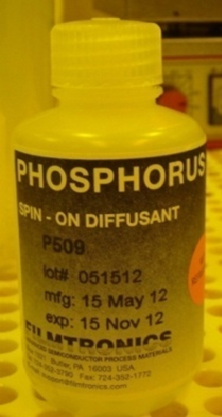
\includegraphics[scale=0.7, trim = 0cm 0cm 0cm
%                             0cm, clip]{./HerstellungBilder/Phosphorus.png}
%                             \caption{Phosphor}
%                            \label{fig:phos}
%                         \end{figure}
% 
%                     \end{minipage}
%                     \begin{minipage}{0.6\textwidth}
% 
%                         \begin{figure}[H]
%                         \hspace{3.5em}
%                             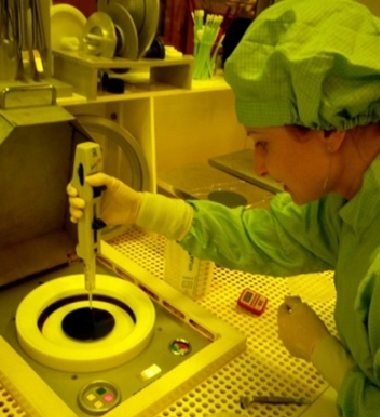
\includegraphics[scale=0.7, trim = 0cm 0cm 0cm
%                             0cm, clip]{./HerstellungBilder/Dotierstoffauftragen.png}
%                             \caption{Auftragen des Dotierstoffes}
%                            \label{fig:aufDot}
%                         \end{figure}
%                     \vspace{-1.5em}
% 
%                     \end{minipage}
% 
%                 \end{tabular}
% 		\end{center}
%     
%     	\vspace{2em}
%     
% 		Um gleichmäßige Verteilung des Dotierstoffes zu bekommen, wurde die 
% 		Auftragung der Phosphorlösung mit einem 
% 		Lackschleuderbeschichtungsapparat (s. Abb.) durchgeführt.\\
%  		Auf einem Drehtisch wird der Wafer zentral justiert und mittels Vakuum
%  		fixiert, damit der Wafer bei der Drehung am Teller gut haftet. Mit Hilfe 
%  		von Dispenser (die zwei	Mal gedrückt wurde) wird der Dotierstoff auf den
%  		Wafer getropft. Danach muss der Wafer sofort in Rotation gebracht werden
%  		, um eine ebenmäßige Dotierstoffschicht zu bekommen. Bei der Rotation 
%  		wird die überflüssige Stoffmenge von der Scheibe weggeschleudert.\\
% 		Es bleibt nur eine sehr dünne Phosphorschicht auf dem Wafer.\\
% 
% 		Bedingungen beim Aufschleudern der Phosphorlösung:\\
% 		Programm 4\\
% 		2500 U/min (Anzeige 250)\\
% 		2 ml Lösung\\
% 
% 		Bemerkung: der Wafer 120503 wurde doppelt mit dem Dotierstoff 
% 		beschichtet (ca. 4 ml).\\
% 		Anschließend wurden alle drei Wafer auf der Heizplatte  15 Minuten lang 
% 		bei 200°C gebacken. Bei diesem Prozessschritt bildet sich ein 
% 		Phosphorglas (Silikat). Dabei wurde eine Dampfwolke beobachtet. \\
% 		Das Ergebnis nach diesem Vorgang ist in der Abbildung \ref{fig:Waf_phos}  
% 		zu sehen.\\   
%     
%         \vspace{2em}
%             
%     		\begin{figure}[H]
% 				\hspace{4.7 cm}
%                 \includegraphics[scale=0.5, trim = 0cm 0cm 0cm 0cm,clip]
%                 	{./HerstellungBilder/StrukturmitPhosphorus.png}
%                   \caption{Wafer bedeckt mit Phosphorglas}
%                 \label{fig:Waf_phos}
%             \end{figure}
%             
%         \vspace{2em}
%             
% 		Eine Sichtkontrolle mit dem Lichtmikroskop hat uns folgendes ausgegeben:
%          
%      	\vspace{2em}
%             
%     		\begin{figure}[H]
% 				\hspace{3.5 cm}
%                 \includegraphics[scale=0.5, trim = 0cm 0cm 0cm 0cm,clip]
%                 	{./HerstellungBilder/Mikroskopbild2.png}
%                   \caption{Bläschen Wafer 01}
%                 \label{fig:blaes}
%             \end{figure}
%       
%      	\vspace{2em}
%      
%     	Zu beobachten war:\\
% 		Bei dem Wafer 02 waren Bläschen stärker, der Wafer 03 hatte fast gar 
% 		keine Bläschen, die Struktur war ebenmäßiger und er enthielt so viel 
% 		Dotierstoff, dass die Fenster kaum zu sehen waren. Der Wafer 01 hatte 
% 		große Bläschen, die ständig Ihre Form verändert haben.
%             
% 		\end{quote}
% 	
% 		2 Diffusionsofen:\\
% 
% 		Jetzt kommen die Wafer in den Diffusionsofen.\\
% 	
% 		Als erstes wurden die Wafer  so in dem Quarzschiffchen einsortiert, dass 
% 		sich die Vorderseiten der Wafer 01 und 02 gegenüber stehen. Wafer 03 
% 		wurde einsam auf der anderen Seite des Quarzschiffchens platziert.
% 	
% 		\vspace{2em}
%     
%     	\begin{center}
%                 \begin{tabular}{ll}
% 
%                 \hspace{-7em}
%                     \begin{minipage}{0.5\textwidth}
%                         \begin{figure}[H]
%                         \hspace{-2em}
%                             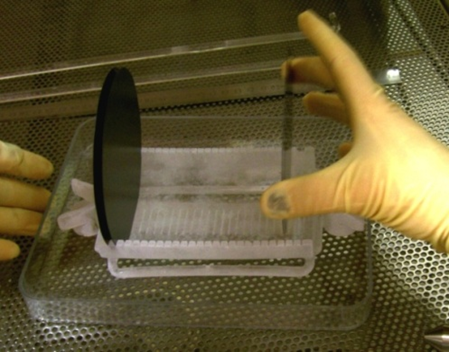
\includegraphics[scale=0.8, trim = 0cm 0cm 0cm
%                             0cm, clip]{./HerstellungBilder/Quarzschiffchen.png}
%                             \caption{Quarzschiffchen}
%                            \label{fig:quarz}
%                         \end{figure}
% 
%                     \end{minipage}
%                     \begin{minipage}{0.75\textwidth}
% 
%                         \begin{figure}[H]
%                         \hspace{8em}
%                             \includegraphics[scale=0.7, trim = 0cm 0cm 0cm
%                             0cm, clip]
%                             {./HerstellungBilder/einbringeninDiffusionsofen.png}
%                             \caption{Einbringen in den Diffusionsofen}
%                            \label{fig:ein_diff}
%                         \end{figure}
%                     \vspace{-1.5em}
% 
%                     \end{minipage}
% 
%                 \end{tabular}
% 		\end{center}
% 	
% 		\vspace{2em}
% 	
% 		Dann wird das Schlitten 65 cm tief im Ofen platziert, damit die Wafer 
% 		sich möglichst in der Ofenmitte befinden. Zum Abschluss wurde 
% 		anschließend noch ein Quarzhohlzylinder in den Ofen geschoben, um die 
% 		Temperaturhaltung zu verbessern.\\
% 		Der Prozess der Diffusion findet unter dem Durchströmen des 
% 		Diffusionsofens mit dem Prozessgas für zehn min. bei der Temperatur von 
% 		1000 °C. 
% 	
% 		\vspace{2em}
%             
%     		\begin{figure}[H]
% 				\hspace{4 cm}
%                 \includegraphics[scale=0.75, trim = 0cm 0cm 0cm 0cm,clip]
%                 	{./HerstellungBilder/diffusionsofen.png}
%                   \caption{Diffusionsofen}
%                 \label{fig:diff_ofen}
%             \end{figure}
%             
%     	\vspace{2em}
% 	
% 		Nach dem Diffusionsprozess verblieben die Wafer noch zum langsamen 
% 		Auskühlen über die Nacht im Ofen.\\
% 	
% 			Nach der Diffusion sieht unsere Struktur so aus wie in Abb. 
% 			\ref{fig:nach_diff_ofen}:
% 	
% 			\vspace{2em}
%             
%     		\begin{figure}[H]
% 				\hspace{4 cm}
%                 \includegraphics[scale=0.7, trim = 0cm 0cm 0cm 0cm,clip]
%                 	{./HerstellungBilder/StrukturnachDiffusionsofen.png}
%                   \caption{Struktur nach Diffusionsofen}
%                 \label{fig:nach_diff_ofen}
%             \end{figure}
%             
%     		\vspace{2em}
% 	
% 		\subsubsection{2. Tag}
% 		
% 			Am zweiten Tag haben wir unsere Wafer aus dem Ofen genommen. Dabei 
% 			haben wir beobachtet, dass der Wafer 03 glänzend und der Wafer 01 
% 			und 02 matt waren. Danach wurden alle Wafer einer Sichtkontrolle 
% 			unter dem Mikroskop unterzogen und  mit dem Photometer wurde die 
% 			Schichtdicke gemessen.\\
% 
% 			Photometer: Das Photometer Ergolux besteht aus einem Mikroskop mit 
% 			einem  Aufsatz, der Licht bestimmter Wellenlängen (zwischen 400 nm 
% 			und 800 nm ) auf den Wafer strahlt und über die Reflexion der 
% 			Lichtquanten der unterschiedlichen Wellenlängen den Aufschluss über 
% 			die Schichtdicke gibt.\\
% 
% 			Zur Kalibrierung muss das Photometer mit einer Musterprobe justiert 
% 			werden(mit dem Flat nach unten):  die Musterprobe (ein nicht 
% 			beschichteter Siliziumwafer) soll auf den Objekthalter so platziert 
% 			werden, damit man die Bildschärfe einstellen kann. Dann startet man 
% 			das Programm  Justage. Danach wird es ohne Musterprobe auf dem 
% 			Objekthalter noch mal gestartet.\\
% 			Nur dann  können wir unsere Wafer messen.\\
% 
% 			Die Messergebnisse für unsere drei Wafer sind in der Tabelle 
% 			\ref{tab:Phosphordicke} zusammengefasst.
% 			
% 			\vspace{2em}
% 
%       		\begin{table}[h]
%      		  \begin{addmargin}[1cm]{3cm}
%      			\centering
%                     \begin{tabular}{|p{2cm}|p{2cm}|p{2cm}|p{2cm}|p{2cm}|p{2cm}|}
%          			\hline
%          			Wafer & oben & mittig & unten & links & rechts\\
%          			\hline 
%         			120501 & 82.3  & 78.1  & 86.8  & 85.4  & 73.2 \\
%                     120503 & 770.1 & 784.8 & 765.3 & 764.8 & 776.2 \\
%                     \hline
%         
%                     \end{tabular}
%               \end{addmargin}
%               \caption{gemessene Phosphorglasdicke in nm}
%               \label{tab:Phosphordicke}
%             \end{table}
% 
%             \vspace{2em}
%             
%             Die Wafer 01 und 02 waren nicht gut messbar! Der Wafer 03  hat 
%             dagegen fast perfekte Messergebnisse. 
%             
%             \vspace{2em}
%     
%     		\begin{center}
%                 \begin{tabular}{ll}
% 
%                 \hspace{-7em}
%                     \begin{minipage}{0.5\textwidth}
%                         \begin{figure}[H]
%                         \hspace{-1em}
%                             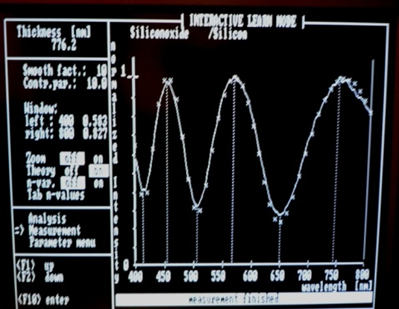
\includegraphics[scale=0.8, trim = 0cm 0cm 0cm
%                             0cm, clip]{./HerstellungBilder/Photometerbild.png}
%                             \caption{Photometerbild}
%                            \label{fig:photobild}
%                         \end{figure}
% 
%                     \end{minipage}
%                     \begin{minipage}{0.7\textwidth}
% 
%                         \begin{figure}[H]
%                         \hspace{5em}
%                             \includegraphics[scale=0.8, trim = 0cm 0cm 0cm
%                             0cm, clip]
%                             {./HerstellungBilder/Photometer.png}
%                             \caption{Das Photometer}
%                            \label{fig:photometer}
%                         \end{figure}
%                     \vspace{-1.5em}
% 
%                     \end{minipage}
% 
%                 \end{tabular}
% 			\end{center}
% 	
% 			\vspace{2em}
% 		
% 			Sichtkontrolle unter dem Lichtmikroskop:\\
% 			Wafer02 und Wafer01:keine klare Struktur(wegen sehr guten 
% 			Diffusion??)
% 		
% 		    \vspace{2em}
%     
%     		\begin{center}
%                 \begin{tabular}{ll}
% 
%                 \hspace{-14em}
%                     \begin{minipage}{0.8\textwidth}
%                         \begin{figure}[H]
%                         \hspace{8em}
%                             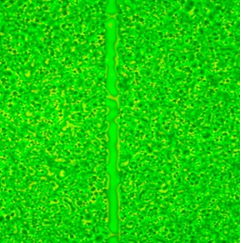
\includegraphics[scale=1.2, trim = 0cm 0cm 0cm
%                             0cm, clip]{./HerstellungBilder/MikroskopW1.png}
%                             \caption{Wafer 01 nach der Diffusion}
%                            \label{fig:diff01}
%                         \end{figure}
% 
%                     \end{minipage}
%                     \begin{minipage}{0.4\textwidth}
% 
%                         \begin{figure}[H]
%                         \hspace{-2em}
%                             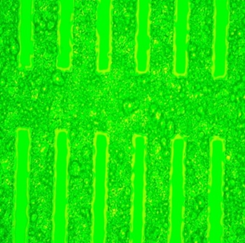
\includegraphics[scale=1.2, trim = 0cm 0cm 0cm
%                             0cm, clip]{./HerstellungBilder/MikroskopW2.png}
%                             \caption{Wafer 02 nach der Diffusion}
%                            \label{fig:diff02}
%                         \end{figure}
%                     \vspace{-1.5em}
% 
%                     \end{minipage}
% 
%                 \end{tabular}
% 			\end{center}
%     
%     		\vspace{2em}
% 			
% 			Wafer03: man kann einen großen Farbunterschied sehen. Die Schicht 
% 			machte optisch einen guten Eindruck, die Struktur ist sehr klar.\\
% 
% 			Ätzen (Entfernen des Phosphorglases):\\
% 
% 			Jetzt wird das Phosphorglas entfernt. Dazu wird zuerst der Wafer01 
% 			in die 2.5%-ige Flusssäure für ca. fünf Minuten lang eingetaucht, 
% 			%um das Phosphorglas von der
% 			Oberfläche zu entfernen. Übrig bleibender Phosphor wurde 
% 			anschließend mit dem Wattestäbchen entfernt und in Di-Wasser 
% 			gesäubert.\\
% 			Da die Flusssäure stark ätzend ist, müssen ein extra dicker 
% 			Schutzanzug, Augenschutz und dickere Handschuhe getragen werden 
% 			(Abbildung \ref{fig:schutzbe}). Nach dem Ätzen prüften wir die Dicke 
% 			mit dem Photometer und stellten fest, dass wir die ganze Schicht 
% 			wegätzten!! Die Sichtkontrolle mit dem Lichtmikroskop zeigte, dass 
% 			Struktur noch da war, deswegen wurde entschieden den Wafer02 für 
% 			Schrägschliff zu verwenden.
%  	
%  			\vspace{2em}
%     
%     		\begin{center}
%                 \begin{tabular}{ll}
% 
%                 \hspace{-14em}
%                     \begin{minipage}{0.8\textwidth}
%                         \begin{figure}[H]
%                         \hspace{5em}
%                             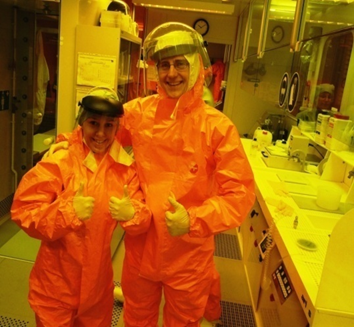
\includegraphics[scale=1.0, trim = 0cm 0cm 0cm
%                             0cm, clip]{./HerstellungBilder/Schutzbekleidung.png}
%                             \caption{Schutzbekleidung}
%                            \label{fig:schutzbe}
%                         \end{figure}
% 
%                     \end{minipage}
%                     \begin{minipage}{0.40\textwidth}
% 
%                         \begin{figure}[H]
%                         \hspace{-4em}
%                             \includegraphics[scale=1.0, trim = 0cm 0cm 0cm
%                             0cm, clip]
%                             {./HerstellungBilder/ArbeitenamLichtmikroskop.png}
%                             \caption{Arbeiten am Lichtmikroskop}
%                            \label{fig:arblicht}
%                         \end{figure}
%                     \vspace{-1.5em}
% 
%                     \end{minipage}
% 
%                 \end{tabular}
% 			\end{center}
%     
%     		\vspace{2em}
%     		
%     		
% 			Der Wafer02 wurde dann zwei Mal geätzt: ein Mal sehr vorsichtig mit 
% 			der 2.5\%-igen Flusssäure nur für eine Minute und danach mit der 
% 			1\%-igen nur für fünf Sekunden, jedes Mal wurde die Dicke gemessen. 
% 			Der Wafer03 wurde  schon mehrmals  geätzt: zwei Mal sehr vorsichtig 
% 			mit der 1\%-igen Flusssäure für eine Minute, dann mit der 1\%-igen 
% 			nur für fünf Sekunden.  Jedes Mal wurde die Dicke kontrolliert. 
% 			Die Ergebnisse der Oxiddickenmessung sind in der Tabelle
% 			\ref{tab:Oxiddicke} dargestellt.
% 			
% 			\vspace{2em}
% 
%       		\begin{table}[h]
%      		  \begin{addmargin}[1cm]{3cm}
%      			\centering
%                     \begin{tabular}{|p{2cm}|p{2cm}|p{2cm}|p{2cm}|p{2cm}|p{2cm}|}
%          			\hline
%          			Wafer & oben & mittig & unten & links & rechts\\
%          			\hline 
%         			120502 & 196.5  & 199.9  & 198   & 205   & 195 \\
%                     120503 & 201 	& 202 	 & 203.7 & 186.7 & 203 \\
%                     \hline
%         
%                     \end{tabular}
%               \end{addmargin}
%               \caption{Oxiddicke}
%               \label{Oxiddicke}
%             \end{table}
% 
%             \vspace{2em}
%             
%             Nach dem Ätzen sieht unsere Struktur folgendermaßen aus:
%             
%             \vspace{2em}
%             
%     		\begin{figure}[H]
% 				\hspace{3.5 cm}
%                   \includegraphics[scale=0.9, trim = 0cm 0cm 0cm 0cm,clip]
%                 	{./HerstellungBilder/KontaktfenstergeaetztundLackentfernt.png}
%                   \caption{Struktur nach dem Ätzen}
%                 \label{fig:nachAetzen}
%             \end{figure}
%             
%     		\vspace{2em}
%     		
%     		Anschließend wurden die Wafer mit dem Stickstoff trocken gepustet 
%     		und für ca. 15 min. bei 200° C auf eine Heizplatte gelegt, um die 
%     		molekulare Flüssigkeitsreste von der Oberfläche des Wafers zu 
%     		entfernen (sie stören die Haftung des Photolacks).\\
%     		
%     		Lithographie:\\
% 
% 			HMDS\\
% 			Die Wafer02 und 03 werden direkt von der Heizplatte in Exikator, 
% 			eine so genannte Vakuumglocke(s. Abb ) mit dem  Haftmittel HMDS 
% 			(Hexamethyldisilazan), gebracht.
%             
%             \vspace{2em}
%     
%     		\begin{center}
%                 \begin{tabular}{ll}
% 
%                 \hspace{-14em}
%                     \begin{minipage}{0.7\textwidth}
%                         \begin{figure}[H]
%                         \hspace{5em}
%                             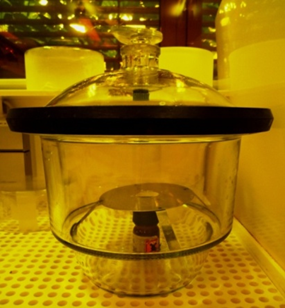
\includegraphics[scale=1.0, trim = 0cm 0cm 0cm
%                             0cm, clip]{./HerstellungBilder/Vakuumglocke.png}
%                             \caption{Vakuumglocke}
%                            \label{fig:vakuumgl}
%                         \end{figure}
% 
%                     \end{minipage}
%                     \begin{minipage}{0.3\textwidth}
% 
%                         \begin{figure}[H]
%                         \hspace{-3em}
%                             \includegraphics[scale=1.0, trim = 0cm 0cm 0cm
%                             0cm, clip]
%                             {./HerstellungBilder/Heizplatte.png}
%                             \caption{Heizplatte}
%                            \label{fig:heizpl}
%                         \end{figure}
%                     \vspace{-1.5em}
% 
%                     \end{minipage}
% 
%                 \end{tabular}
% 			\end{center}
%     
%     		\vspace{2em}
%     		
%     		Es wird das Vakuum für 30 Sekunden lang abgepumpt, HMDS verdampft 
%     		und lagert sich an der Oberfläche des Wafers ab. Es wird ca. fünf 
%     		Minuten beschichtet, danach wird das Druckventil sehr langsam 
%     		gedreht und der Druck abgelassen. Anschließend werden die Wafer 
%     		für eine Minute bei 120°C auf die Heizplatte gelegt.\\
% 
% 			Belacken und Softbake:\\

			Nachdem die Wafer getrocknet waren, wurden sie mit einem Positivlack 
			AZ 5214 beschichtet (s.Abb  und ). Beim Drehen der Schleuder, wenn 
			sich der Lack ausbreitet, beobachtet man die farbigen Wellen. Es 
			sind die Interferenzwellen von den Lackschichten. Je länger die 
			Schleuderzeit ist, desto gleichmäßiger ist die Lackschicht.
    		
    		\vspace{2em}
    
    		\begin{center}
                \begin{tabular}{ll}

                \hspace{-14em}
                    \begin{minipage}{0.7\textwidth}
                        \begin{figure}[H]
                        \hspace{5em}
                            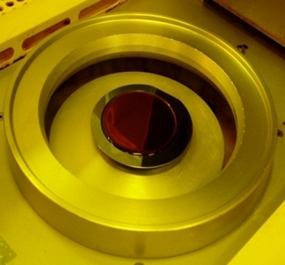
\includegraphics[scale=1.0, trim = 0cm 0cm 0cm
                            0cm, clip]{./HerstellungBilder/BeschichtungdesWafers.png}
                            \caption{Beschichtung des Wafers}
                           \label{fig:Beschwaf}
                        \end{figure}

                    \end{minipage}
                    \begin{minipage}{0.3\textwidth}

                        \begin{figure}[H]
                        \hspace{-1em}
                            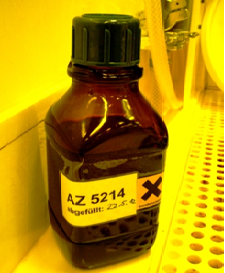
\includegraphics[scale=1.0, trim = 0cm 0cm 0cm
                            0cm, clip]
                            {./HerstellungBilder/Lackflasche.png}
                            \caption{Lackflasche}
                           \label{fig:lackfl}
                        \end{figure}
                    \vspace{-1.5em}

                    \end{minipage}

                \end{tabular}
			\end{center}
    
    		\vspace{2em}
    		
    		Nach dem Lackieren muss der Wafer 30 Minuten lang in der halboffenen 
    		Schachtel ruhen, damit die Gasbläschen rauskommen und der Lack in 
    		die kleinsten Rauigkeiten der Oberfläche eindringen kann. 
    		Anschließend wurden die Wafer bei 90°C zwei Minuten auf der 
    		Heizplatte erhitzt, um den Lack zu fixieren. Sehr wichtig, dass die 
    		Wafer sehr langsam abkühlen müssen!\\

			Belichten mit der KF-Maske:\\
			Das Belichten des Wafers erfolgt auf dem Maskenjustierer(s.Abb.):
			Dieser Lithographie-Apparat hat die Belichtungshaube, darunter ist 
			der Waferhalter und Maskenhalter,  Mikroskop mit einer CCD-Kamera 
			und einem Bildschirm.
			Ganz wichtig ist es, dass die Maske und der Wafer genau übereinander 
			liegen, damit der Wafer an den nötigen Stellen belichtet werden kann
			.\\
 			Als erstes wurde Maskenjustierer angeschaltet und die Lampe 
 			vorgewärmt. Auf dem Bildschirm kann man die unten erscheinenden 
 			Anleitungen befolgen. Weiter wurde die Maske geladen und mit dem 
 			Vakuum festgehalten. Die KF-Maske wurde genau an der AA-Maske 
 			justiert(man kann die Justierung in der Abbildung 
 			\ref{fig:Justiervorgang} sehen, wo die Kreuze übereinanderliegen). 
 			
 			\vspace{2em}
    
    		\begin{center}
                \begin{tabular}{ll}

                \hspace{-14em}
                    \begin{minipage}{0.6\textwidth}
                        \begin{figure}[H]
                        \hspace{2em}
                            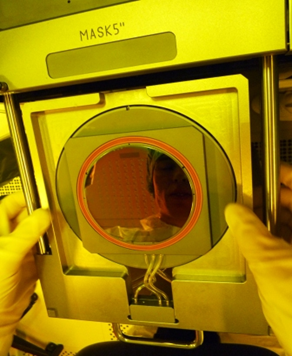
\includegraphics[scale=1.0, trim = 0cm 0cm 0cm
                            0cm, clip]{./HerstellungBilder/Maskenjustierer.png}
                            \caption{Justierung der Maske}
                           \label{fig:just}
                        \end{figure}

                    \end{minipage}
                    \begin{minipage}{0.6\textwidth} 

                        \begin{figure}[H]
                        \hspace{-1em}
                            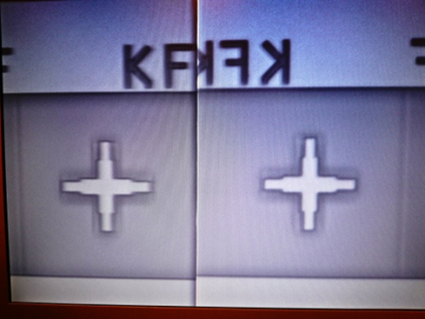
\includegraphics[scale=0.9, trim = 0cm 0cm 0cm
                            0cm, clip]
                            {./HerstellungBilder/Justiervorgang.png}
                            \caption{Justiervorgang}
                           \label{fig:Justiervorgang}
                        \end{figure}
                    \vspace{-1.5em}

                    \end{minipage}

                \end{tabular}
			\end{center}
    
    		\vspace{2em}
    		
    		Der Wafer wurde ausgerichtet, mit dem Vakuum festgehalten und 
    		hineingeschoben. Dann justiert man den Wafer so, dass er genau unter 
    		der Maske liegt (s.Abb. \ref{fig:just}).\\

			Danach drückt man die Taste Exposition und der Wafer wird durch die 
			Maske belichtet. Das Licht befindet sich im UV-Bereich. Bei dem 
			Belichtungsprogramm gibt es verschiedene Belichtungsarten, wir haben 
			uns für die Soft-Kontakt-Belichtungsart entschieden, weil es die 
			schonendste Methode ist. Der Wafer 02 wurde vier Sekunden lang
			belichtet. Der Moment der Belichtung ist in der Abbildung 
			\ref{fig:belichtung} zu sehen.
    		
    		\vspace{2em}
    
    		\begin{center}
                \begin{tabular}{ll}

                \hspace{-14em}
                    \begin{minipage}{0.6\textwidth}
                        \begin{figure}[H]
                        \hspace{2em}
                            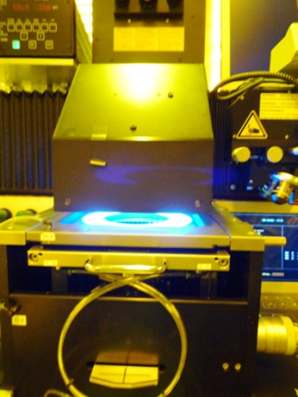
\includegraphics[scale=1.0, trim = 0cm 0cm 0cm
                            0cm, clip]{./HerstellungBilder/Belichtungsvorgang.png}
                            \caption{Belichtungsvorgang}
                           \label{fig:belichtung}
                        \end{figure}

                    \end{minipage}
                    \begin{minipage}{0.6\textwidth} 

                        \begin{figure}[H]
                        \hspace{-1em}
                            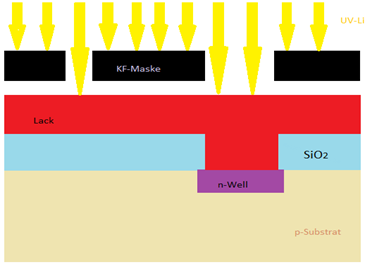
\includegraphics[scale=0.9, trim = 0cm 0cm 0cm
                            0cm, clip]
                            {./HerstellungBilder/DerMomentderBelichtung.png}
                            \caption{Belichtung}
                           \label{fig:belichtung2}
                        \end{figure}
                    \vspace{-1.5em}

                    \end{minipage}

                \end{tabular}
			\end{center}
    
    		\vspace{2em}
    		
    		Die durchsichtigen Bereiche der Maske lassen das Licht durch und der 
    		Wafer wird belichtet.\\
			Durch das Belichten wird der Lack härter. An den Stellen, die nicht
			belichtet wurden, wird der Lack später mit einer Rohm-Haas Lösung 
			abgezogen.\\
			Die Belichtungszeit stimmte für den Wafer02, deswegen wurde der
			Wafer03 auch mit dieser Zeit belichtet. Leider wurde beim Justieren 
			der Wafer03 ein Stückchen Lack an der Maske angeklebt. Wir haben sofort überlegt, ob es beim Entwickeln zu den Fehlern kommen kann.

			Entwickeln und Hardbake: 

			Nach dem Belichtungsprozess wurde der Lack möglichst schnell mit 
			Hilfe von Entwickler Rohm-Haas entfernt. Die Wafer wurden 60 
			Sekunden lang in dieser Lösung gespült.\\
			Nach dem Entwicklungsprozess muss der Entwickler ganz schnell weg 
			von der Waferoberfläche und sehr gründlich mit dem Wasser abgespült 
			werden (s. Abb. \ref{fig:entw}).\\
			Um den restlichen Lack gegen Ätzmittel noch resistenter zu machen:
			Hardbake fünf Minuten lang, 120 °C .
			
			\vspace{2em}
    
    		\begin{center}
                \begin{tabular}{ll}

                \hspace{-14em}
                    \begin{minipage}{0.6\textwidth}
                        \begin{figure}[H]
                        \hspace{2em}
                            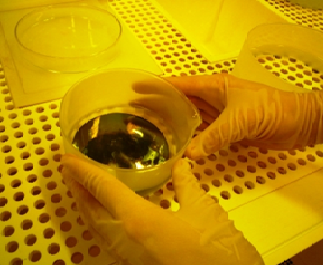
\includegraphics[scale=1.0, trim = 0cm 0cm 0cm
                            0cm, clip]{./HerstellungBilder/Entwickeln.png}
                            \caption{Entwickeln}
                           \label{fig:entw}
                        \end{figure}

                    \end{minipage}
                    \begin{minipage}{0.6\textwidth} 

                        \begin{figure}[H]
                        \hspace{0em}
                            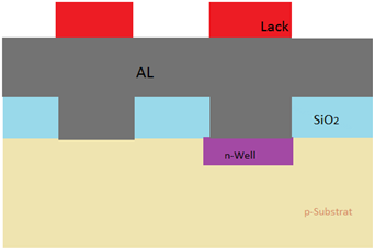
\includegraphics[scale=0.9, trim = 0cm 0cm 0cm
                            0cm, clip]
                            {./HerstellungBilder/NachdemEntwickeln.png}
                            \caption{Nach dem Entwickeln}
                           \label{fig:nachentw}
                        \end{figure}
                    \vspace{-1.5em}

                    \end{minipage}

                \end{tabular}
			\end{center}
    
    		\vspace{2em}
    		
    		Sichtkontrolle:\\

			Mit dem Lichtmikroskop: Nun sollen die Wafer mit dem Mikroskop 
			untersucht werden. Wie wir es schon erwartet haben, der angeklebte 
			Lack hat sich bemerkbar gemacht: Die Struktur ist nicht mehr sehr 
			deutlich zu sehen, viele untergeätzte Stellen:
			
            \vspace{2em}

    		\begin{figure}[H]
				\hspace{3 cm}
                  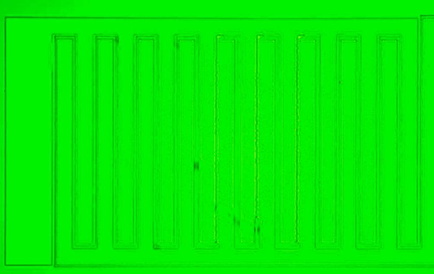
\includegraphics[scale=0.9, trim = 0cm 0cm 0cm 0cm,clip]
                	{./HerstellungBilder/Mikroskopbild3.png}
                  \caption{Nach dem Entwickeln}
                \label{fig:nachentwickelnwaf}
            \end{figure}

    		\vspace{2em}
    		
    		Dektak-Messung:

			Nun wurden die Lackdicken von den Wafern 02 und 03 am Dektak 
			gemessen.\\
			Der Dektak ist ein Profilometer mit dem sich die mikroskopische 
			Oberflächenrauigkeit ermitteln lässt.\\ 
			Ein Mal haben wir über dem p- und das andere Mal über dem n-Pad 
			gemessen:\\

			\vspace{2em}

    		\begin{figure}[H]
				\hspace{-1.5 cm}
                  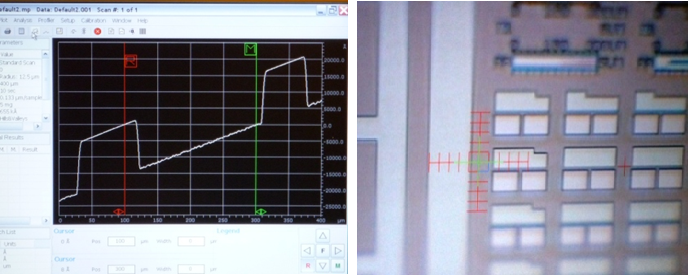
\includegraphics[scale=1, trim = 0cm 0cm 0cm 0cm,clip]
                	{./HerstellungBilder/MessungenamDektak.png}
                  \caption{Messungen am Dektak}
                \label{fig:Dektak}
            \end{figure}

    		\vspace{2em}
    		
    		Die Tabelle \ref{tab:Lackdickenmess} zeigt das Ergebnis:
    		
    		\vspace{2em}

      		\begin{table}[h]
     		  \begin{addmargin}[3cm]{3cm}
     			\centering
                   \begin{tabular}{|p{3cm}|p{3cm}|p{3cm}|}
         			\hline
         			Wafer & p-Pad & n-Pad\\
         			\hline
        			120502 & 1.5 µm     & 185 nm\\
        			\hline
                    120503 & 1.55 µm 	& 182 nm\\
                    \hline

                    \end{tabular}
              \end{addmargin}
              \caption{Lackdickenmessung}
              \label{tab:Lackdickenmess}
            \end{table}

            \vspace{2em}

			Ätzen:\\

			Diesmal wurde das Ätzen vorsichtig mehrmals durchgeführt. Dafür 
			haben wir 1\%-ige gepuffte Flusssäure BHF (HF/NH3F) benutzt. Jeder 
			Wafer wurde in dieser Lösung für ca. eine min. eingetaucht und 
			sofort mit Di-Wasser abgespült.
			
			\vspace{2em}

    		\begin{figure}[H]
				\hspace{3 cm}
                  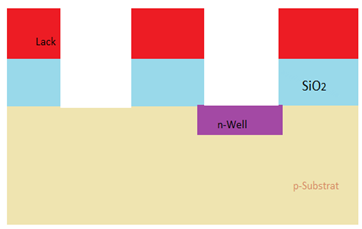
\includegraphics[scale=1, trim = 0cm 0cm 0cm 0cm,clip]
                	{./HerstellungBilder/StrukturnachdemAetzen2.png}
                  \caption{nach dem erneuten Ätzen}
                \label{fig:ernAetz}
            \end{figure}

    		\vspace{2em}
			
			Zwischen den Ätzungen haben wir ständig die Oxiddicke mit Dektak 
			kontrolliert. Die Dektakmessung zeigte uns, dass der Ätzvorgang sehr
			langsam abläuft. Die Kontrolle am Lichtmikroskop hat aber folgendes 
			gezeigt:\\
			Wafer03 wurde total übergeätzt! Starke Dotierung wurde als mögliche 
			Ursache dafür vermutet.
			
			\vspace{2em}

    		\begin{figure}[H]
				\hspace{-0.7 cm}
                  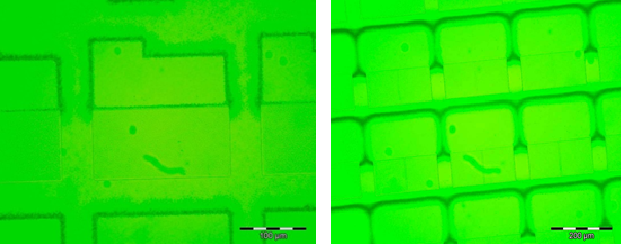
\includegraphics[scale=1, trim = 0cm 0cm 0cm 0cm,clip]
                	{./HerstellungBilder/LichtmikroskopbilderW23.png}
                  \caption{erneute Aufnahme mit dem Lichtmikroskop}
                \label{fig:ernLichtmi}
            \end{figure}
            
    		\vspace{2em}
    		
    		
    		Da der Wafer03 übergeätzt wurde, haben wir entschieden, dass es 
    		keine AL-Metallisierung bei ihm durchgeführt wird.\\
			Dagegen Wafer02 war in Ordnung, nur die Kanten waren unscharf(s. 
			Abb. \ref{fig:ernLichtmi})

			Lack entfernen:

			Als letztes wurde Lack von den Wafern 02 und 03 mit dem Aceton 
			entfernt.\\
			Nach dem Lithographie-Schritt sieht unsere Struktur folgendermaßen 
			aus:
    		
    		\vspace{2em}

    		\begin{figure}[H]
				\hspace{3 cm}
                  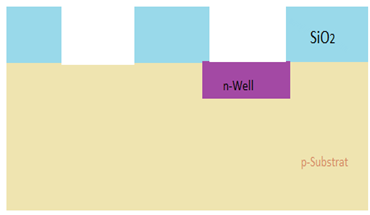
\includegraphics[scale=1, trim = 0cm 0cm 0cm 0cm,clip]
                	{./HerstellungBilder/KontaktfenstergeaetztundLackentfernt.png}
                  \caption{Kontaktfenstermaske geätzt und entfernt}
                \label{fig:Konfengeaetzt}
            \end{figure}
            
    		\vspace{2em}
    		
			Anschließend wurden von allen drei Wafer die organische Stoffe mit 
			dem Ätzmittel Caro's Etch entfernt.
			
		\end{quote}
		
		\subsubsection{3.Tag}
		\begin{quote}
			
		PVD, Metallisieren:\\

 		PVD (physical vapour deposition) ist die physikalische 
 		Gasphasenabscheidung, die für die vakuumbasierten  Beschichtung mit 
 		Aluminium verwendet wird. Die Abbildung --- zeigt die schematische 
 		Darstellung eines PVD-Verdampfungsverfahrens.
 		
 		\vspace{2em}

    		\begin{figure}[H]
				\hspace{1.5 cm}
                  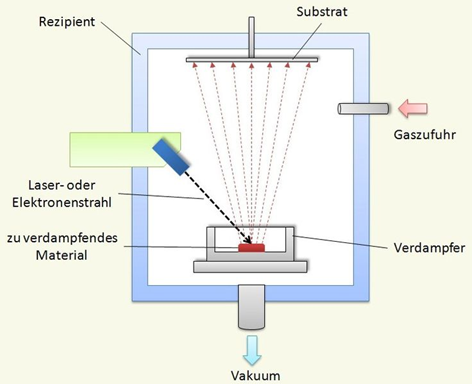
\includegraphics[scale=1, trim = 0cm 0cm 0cm 0cm,clip]
                	{./HerstellungBilder/SchematischeDarstellungeinesPVD-Verdampfungsverfahrens.png}
                  \caption{PVD-Verdampfungsverfahren}
                \label{fig:PVD}
            \end{figure}
            
    	\vspace{2em}
    	
    	Quelle: http://de.wikipedia.org/wiki/Physikalische_Gasphasenabscheidung
 		
 		Das abzuscheidende Material (Target) liegt in fester Form vor. Mit dem 
 		Laser- oder Elektronenstrahl, der von einer Elektronenquelle geschossen 
 		werden, werden die Ionen oder Elektronen durch ein elektromagnetisches 
 		System auf das Target umgelenkt und das Material wird verdampft.\\

		Das  Material verdampft  wegen des sehr niedrigen Druckes und der 
		Energie der Elektronen. Es bildet sich ein Dampf, der durch elektrische 
		Felder durch die Kammer geführt wird. Dabei trifft  der Dampf auf die zu 
		beschichtenden Teile und es kommt zu einer Schichtbildung.\\
		Die Elektronenstrahlkanonen setzen ein Vakuum voraus, deswegen wurde das 
		Vakuum in der Bedampfungsanlage (s. Abb. \ref{fig:Bedampf}) über die 
		Nacht abgepumpt.
 		
 		\vspace{2em}

    		\begin{figure}[H]
				\hspace{0 cm}
                  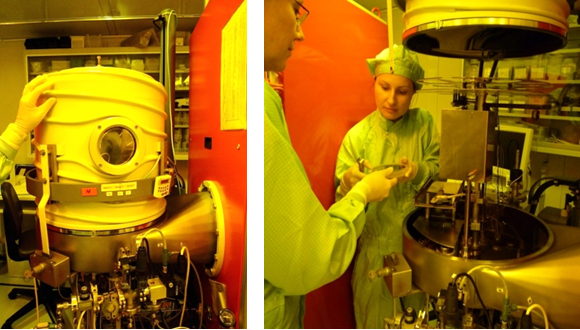
\includegraphics[scale=1, trim = 0cm 0cm 0cm 0cm,clip]
                	{./HerstellungBilder/Bedampfungsanlage.png}
                  \caption{Bedampfungsanlage}
                \label{fig:Bedampf}
            \end{figure}
            
    	\vspace{2em}
 		
 		
		Bevor der Wafer in die PVD-Anlage platziert wird, wurde die 
		Waferoberfläche noch Mal mit einer  1\%-igen HF-Lösung (HF-Dip) für 15 
		Sekunden gereinigt. Diese Lösung dient dazu, die neuentstandene 
		Oxidschicht zu entfernen.\\
		Danach wurde unser einziger Wafer02 in den PVD-Apparat mit der 
		Vorderseite nach unten eingelegt. Außer des Einlegens des Wafers wurden 
		alle Schritte mit Hilfe der Steuerungstasten automatisch ausgeführt.\\
		Dann wird das Programm eingestellt und der PVD-Prozess fängt an. Die 
		aufzusputternde AL-Schicht soll 500 nm betragen.\\

		Da der PVD-Prozess 30 Minuten dauerte, wurden inzwischen Wafer 01 und 03 
		noch Mal mit Phosphorus beschichtet. Anschießend wurden die Wafer 30 
		Minuten lang mit 200°C gebacken. Diese Improvisation war notwendig, da 
		die beiden Wafer keine Oxidschicht mehr hatten.\\
		Nach PVD wurde Wafer02 mit einer Salpetersäure zehn Minuten lang 
		behandelt.
		
		\vspace{2em}

    		\begin{figure}[H]
				\hspace{3 cm}
                  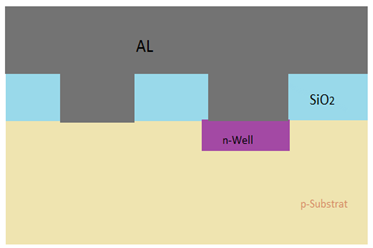
\includegraphics[scale=1, trim = 0cm 0cm 0cm 0cm,clip]
                	{./HerstellungBilder/Wafer02NachderMetallisierung.png}
                  \caption{Metallisierung}
                \label{fig:metall}
            \end{figure}
            
    	\vspace{2em}
    	
    	Wafer für den Schrägschliff brechen:\\
 
		Weiter wurden Wafer 01 und 03 für den Schrägschliffwinkel gebrochen.\\
		Die Wafer wurden zuerst in der Mitte angeritzt. Unter den Wafer an 
		dieser angeritzten Stelle haben wir eine alte Probe gelegt und dann 
		durch einen leichten Druck den Wafer zum Brechen gebracht .Es ist leicht 
		durchzuführen, da Silizium entlang der Kristallrichtung bricht. Die 
		entstandenen Proben haben die Abmessungen ca. 5 X 5 mm2. Die Proben 
		wurden in den vormarkierten Kästchen gelegt.\\

		Lithographie mit der AL-Maske:\\

		Nun werden die typischen Lithographie-Schritte bei leicht abgeänderten 
		Bedingungen noch Mal durchgeführt.\\

		Prebake, Belacken, Softbake: \\

		Die Flüssigkeitsreste werden entfernt, indem die Wafer 30 min. lang bei 
		140°C auf der Heizplatte liegen bleiben.\\

		Danach wird der Wafer 02 mit einem Lack  Az 52/4 beschichtet und 
		anschließend zwei Minuten lang bei 95°C getrocknet. Die Ruhezeit 
		beträgt eine Stunde.\\

		Belichten mit Al-Maske:\\

		Der Wafer02 wird genau so belichtet, wie oben schon beschrieben wurde 
		(s. Lithographie am Tag2),(s. Abb.\ref{fig:belichten3}) Bemerkung: Die Al-Maske wurde 
		auch nach AA-Maske justiert, und die Belichtungszeit beträgt jetzt nur 3
		,7 Sekunden, da Aluminium glänzend ist und Licht reflektiert.\\

 		Danach wurde der Lack mit der Rohm Haas-Lösung entwickelt 
 		(Abb.\ref{fig:nachAetzen}).
    	
    	\vspace{2em}
    
    		\begin{center}
                \begin{tabular}{ll}

                \hspace{-14em}
                    \begin{minipage}{0.8\textwidth}
                        \begin{figure}[H]
                        \hspace{6em}
                            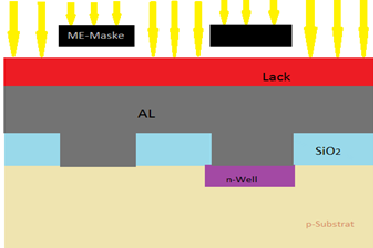
\includegraphics[scale=0.9, trim = 0cm 0cm 0cm
                            0cm, clip]{./HerstellungBilder/BelichtendurchMEMaske.png}
                            \caption{Belichten}
                           \label{fig:belichten3}
                        \end{figure}

                    \end{minipage}
                    \begin{minipage}{0.6\textwidth} 

                        \begin{figure}[H]
                        \hspace{1em}
                            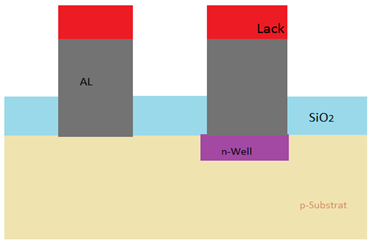
\includegraphics[scale=0.9, trim = 0cm 0cm 0cm
                            0cm, clip]
                            {./HerstellungBilder/StrukturnachdemAetzvorgang.png}
                            \caption{Struktur nach dem Ätzvorgang}
                           \label{fig:nachAetzen}
                        \end{figure}
                    \vspace{-1.5em}

                    \end{minipage}

                \end{tabular}
			\end{center}
    
    		\vspace{2em}
    		
    		Sichtkontrolle:\\

			Nun soll der Wafer mit dem Lichtmikroskop untersucht werden. Wenn 
			der Lack nicht bis zum Ende entwickelt wurde, kann man die 
			Lichtinterferenz sehen, was wir auch in den kleinen Mengen gesehen 
			haben.\\

			Dektak-Messung ergab, dass die Dicke nur 1,36 µm ist, aber wir 
			brauchen mindestens 1,5 µm. Deswegen wurde entschieden, noch Mal 
			zehn Sekunden lang Nachentwicklung zu machen. Nächste Messung ergab 
			1,35 µm. Danach wurde der Wafer noch mit dem Photometer untersucht 
			und es sprach nichts dagegen, dass der Lack nicht entwickelt wurde.\\ 

			Ätzen:\\

			Vor dem Ätzen wird der Wafer noch für fünf Minuten lang auf die 
			Heizplatte bei 140°C gelegt.\\
			Der Ätzvorgang wird diesmal mit einer Ätzmischung aus der 
			Phosphorsäure, Essigsäure, Wasser und der Salpetersäure durchgeführt
			(H3PO4 +H2O+HNO3). Es wurde mehrmals in der Zehner-Intervall 
			(je zehn Sekunden in der Lösung) geätzt, danach wurde schnell in das 
			Di-Wasser eingetaucht und abgespült.  Nach der Sicht wurde beurteilt
			, ob die Al-Schicht weggeätzt wurde. Beobachtung: viel 
			Bläschen.
			
			\vspace{2em}

    		\begin{figure}[H]
				\hspace{3 cm}
                  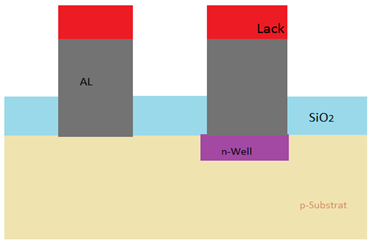
\includegraphics[scale=1, trim = 0cm 0cm 0cm 0cm,clip]
                	{./HerstellungBilder/StrukturnachdemAetzvorgang.png}
                  \caption{Struktur nach dem Ätzvorgang}
                \label{fig:Strukaetz}
            \end{figure}
            
    		\vspace{2em}
    		
    		Kontrolle mit dem Lichtmikroskop: \\

			Die Untersuchung mit dem Lichtmikroskop hat uns gute Bilder 
			geliefert: Die Kontakte sehen gut aus, nur ein wenig untergeätzt 
			(dunkler Rand, s. Abb \ref{fig:darlicht}).
			
			\vspace{2em}

    		\begin{figure}[H]
				\hspace{3 cm}
                  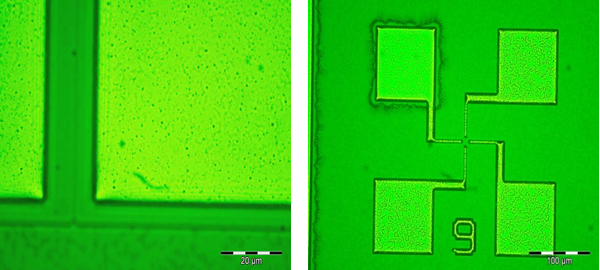
\includegraphics[scale=1, trim = 0cm 0cm 0cm 0cm,clip]
                	{./HerstellungBilder/Lichtmikroskopbilder4.png}
                  \caption{Darstellung mit dem Lichtmikroskop}
                \label{fig:darlicht}
            \end{figure}
            
    		\vspace{2em}
		
			Photolack entfernen:\\

			Als letzter Schritt wird der Lack entfernt. Diesmal wird er in das 
			Aceton für drei Minuten eingetaucht, danach sehr schnell mit Wasser 
			gesäubert. Anschließend wurde unser Wafer in einem Ultraschallbad 
			gereinigt(Abb.\ref{fig:ultra}).
			
			\vspace{2em}
    
    		\begin{center}
                \begin{tabular}{ll}

                \hspace{-14em}
                    \begin{minipage}{0.7\textwidth}
                        \begin{figure}[H]
                        \hspace{7.7em}
                            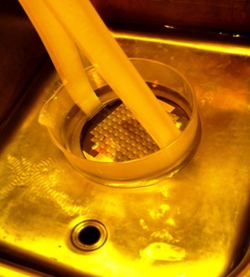
\includegraphics[scale=1, trim = 0cm 0cm 0cm
                            0cm, clip]{./HerstellungBilder/Ultraschalbad.png}
                            \caption{Ultraschallbad}
                           \label{fig:ultra}
                        \end{figure}

                    \end{minipage}
                    \begin{minipage}{0.5\textwidth} 

                        \begin{figure}[H]
                        \hspace{0em}
                            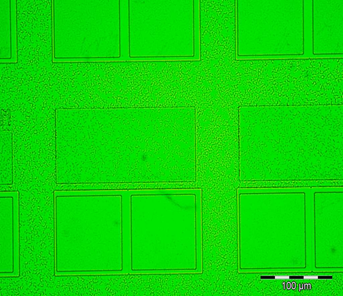
\includegraphics[scale=0.9, trim = 0cm 0cm 0cm
                            0cm, clip]
                            {./HerstellungBilder/LichtmikroskopbildEndstruktur.png}
                            \caption{Lichtmikroskopaufnahme}
                           \label{fig:auflicht}
                        \end{figure}
                    \vspace{-1.5em}

                    \end{minipage}

                \end{tabular}
			\end{center}
    
    		\vspace{2em}
    		
    		Am Ende haben wir unseren Wafer noch Mal am Lichtmikroskop 
    		untersucht. Die Ergebnisse waren gut: Kanten sind sehr glatt, 
    		sehr gute, klare Struktur (s. Abb. \ref{fig:auflicht}).\\

			Enddickenmessung:\\

			Die Aluminiumdickenmessung mit dem Profilometer ergab die Werte 
			zwischen 470 nm und 490 nm, was dem theoretisch erwarteten Wert von
			500 nm entsprach. 

			Tempern:\\ 

			Dieser Temperaturprozess dient der Verbesserung der Kontakte  
			zwischen dem Aluminium und dem Substrat. Dafür wurde der Wafer bei 
			400°C für 30 Minuten im Ofen erhitzt.\\

			Unser Endergebnis, also ein pn-Übergang, ist schematisch  in der 
			Abbildung \ref{fig:end} dargestellt. 
    		
    		\vspace{2em}

    		\begin{figure}[H]
				\hspace{3 cm}
                  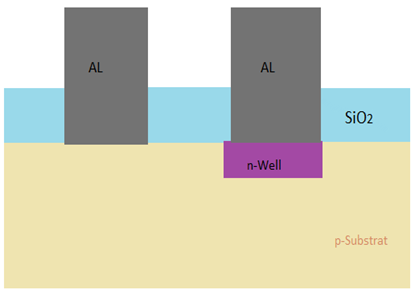
\includegraphics[scale=1, trim = 0cm 0cm 0cm 0cm,clip]
                	{./HerstellungBilder/Endstruktur.png}
                  \caption{Endstruktur}
                \label{fig:end}
            \end{figure}
            
    		\vspace{2em}
    		

    		\begin{figure}[H]
				\hspace{3 cm}
                  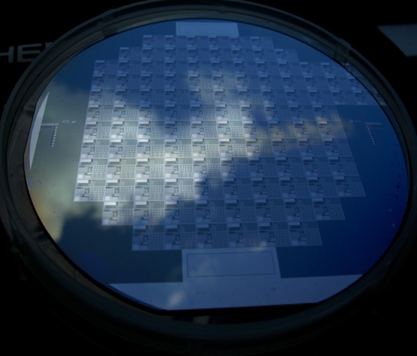
\includegraphics[scale=1, trim = 0cm 0cm 0cm 0cm,clip]
                	{./HerstellungBilder/EndergebnisWafer120502.png}
                  \caption{Endstruktur Wafer}
                \label{fig:endwaf}
            \end{figure}
            
    		\vspace{2em}
    		
			\end{quote}
    	
    	\subsubsection{4.Tag}
    	\begin{quote}
    	
    		Um die pn-Übergangstiefe zu messen wurden unsere Proben zuerst 
    		geschliffen (weil die pn-Tiefe nicht direkt mit dem Mikroskop 
    		gemessen werden kann).\\
			Jede Probe wird zuerst auf einen Support geklebt, indem man den 
			Support auf einer Heizplatte bei 120° heizt und der spezielle 
			Klebstoff darauf geschmolzen wird (s.Abb. \ref{fig:kleb}).
    	
    		\vspace{2em}
    		
    		\begin{figure}[H]
				\hspace{3 cm}
                  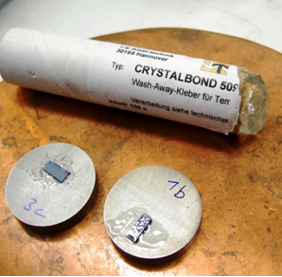
\includegraphics[scale=1, trim = 0cm 0cm 0cm 0cm,clip]
                	{./HerstellungBilder/KlebstoffunddieProben.png}
                  \caption{Klebstoff}
                \label{fig:kleb}
            \end{figure}
            
    		\vspace{2em}
    		
    		Die Proben werden dann mit einem Schleifmittel (Suspension DP aus 
    		Diamantpartikeln) fünf Minuten lang geschliffen(s. 
    		Abb ref{fig:schlei}), so dass sie am Rand einen Schrägschliff 
    		bekommen. Danach werden die Proben abgespült und getrocknet.
    	
   			\vspace{2em}
    		
    		\begin{figure}[H]
				\hspace{3 cm}
                  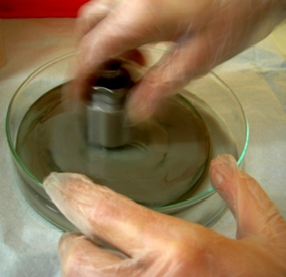
\includegraphics[scale=1, trim = 0cm 0cm 0cm 0cm,clip]
                	{./HerstellungBilder/Schleifen.png}
                  \caption{Schleifen}
                \label{fig:schlei}
            \end{figure}
            
    		\vspace{2em}   	
    	
    		Dekoration:\\

			Zuerst wurde mit der HF:CH3COOH:HNO3 (1:4:5) Lösung versucht, die 
			Probe zu dekorieren. Es hat nicht funktioniert und deswegen wurde 
			entschlossen, mit der Verkupferung zu versuchen.\\

			Die Dekoration der Proben wird dann im Reinraum mit einer Lösung aus 
			zwei Gramm CuSO4 , fünf ml HF(40\%) und 100ml H2O dekoriert. Am 
			Anfang des Vorgangs liegen die Proben in der Lösung mit der 
			Vorderseite nach oben. Sie werden dann mit zwei "Schwanenhals"-
			Lampen drei bis fünf Sekunden belichtet, damit das Licht den Prozess
			aktivieren kann.
    		
    		\vspace{2em}
    		
    		\begin{figure}[H]
				\hspace{3 cm}
                  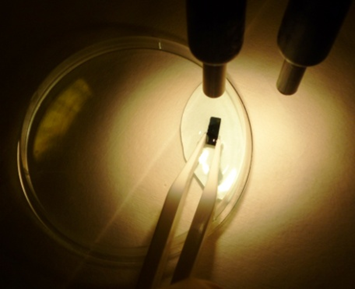
\includegraphics[scale=1, trim = 0cm 0cm 0cm 0cm,clip]
                	{./HerstellungBilder/Verkupferung.png}
                  \caption{Verkupferung}
                \label{fig:verk}
            \end{figure}
            
    		\vspace{2em}
    		
    		Die Kupferlösung wird auf der Oberfläche der Probe an dem 
    		angeschliffenen Gebiet aufgetragen. Da die Kupfermischung einen 
    		Mangel an den Elektronen hat, lagert sich diese Lösung an dem 
    		n-Gebiet, wo es mehr Elektronen gibt. Deswegen erscheint die 
    		n-leitende Seite des pn-Übergangs heller getönt als die p-leitende 
    		Seite (s.Abb. \ref{fig:dek}). Anschließend werden die Proben mit dem Aceton 
    		gereinigt.
    		
    		\vspace{2em}
    		
    		\begin{figure}[H]
				\hspace{3 cm}
                  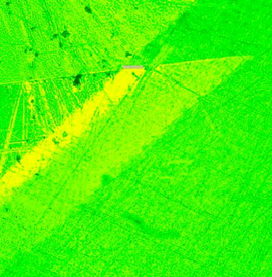
\includegraphics[scale=1, trim = 0cm 0cm 0cm 0cm,clip]
                	{./HerstellungBilder/DekorationunterdemLichtmikroskop.png}
                  \caption{Dekoration unterm Lichtmikroskop}
                \label{fig:dek}
            \end{figure}
            
    		\vspace{2em}
    		
    		
			Unter dem Mikroskop ist dieser Unterschied gut sichtbar und lässt 
			sich ohne Schwierigkeiten auswerten (es wird die Länge der 
			Verkupferung gemessen):\\
			$Wafer01_a: 80µm$\\
			$Wafer01_b: 75µm$\\
			
			Dektak-Messung:\\

			$Wafer01_b:$\\

			Tiefe 7,0 µm, Länge 300 µm\\
			Tiefe 6,9 µm, Länge 300 µm\\

			$Wafer01_a$:\\

			Tiefe 6,2 µm, Länge 300 µm\\
			Tiefe 5,7 µm, Länge 300 µm\\
			
			Daraus kann man die Junctions-Tiefe ausrechnen:
			
			\vspace{2em}
    		
    		\begin{figure}[H]
				\hspace{3 cm}
                  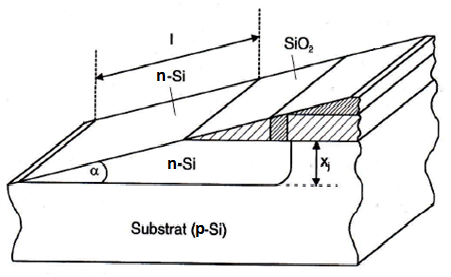
\includegraphics[scale=1, trim = 0cm 0cm 0cm 0cm,clip]
                	{./HerstellungBilder/SchematischeDarstellungzumAusrechnenderpnTiefe.png}
                  \caption{Darstellung zur Tiefenbestimmung}
                \label{fig:dartief}
            \end{figure}
            
    		\vspace{2em}
			
			Nach  der Beziehung $x_j=sin \alpha$, haben wir folgende Ergebnisse 
			ausgerechnet:\\

			$Wafer01_b:$\\
			1,52 µm \\
			1,65 µm \\

			$Wafer01_a:$\\

			1,76 µm\\ 
			1,7 µm\\

 
			Die ausgerechneten Werte entsprechen unseren Erwartungen, was ein 
			Indiz dafür ist, dass die Prozessschritte richtig gemacht wurden.\\ 

			So endet unser Praktikum im Reinraum. \\


			Schlussbetrachtung:\\

			Als Ergebnis unserer Tätigkeit haben wir nur einen Wafer mit vielen 
			pn-Übergängen angefertigt. Die anderen Wafer haben wir für den 
			Schrägschliff verwendet.\\

			Insgesamt haben alle Teilnehmer durch diese vier Tage im 
			Reinraumlabor viel Wissen über die Arbeit im Reinraum, den Umgang 
			mit gefährlichen Stoffen, Arbeit am Mikroskop und Profilometer, und 
			die Herstellungsprozesse eines pn-Übergangs erworben.\\
			Praktische Arbeit hat unser theoretisches Wissen sehr bereichert.
    		
    		\vspace{2em}
    		
    		\begin{figure}[H]
				\hspace{0 cm}
                  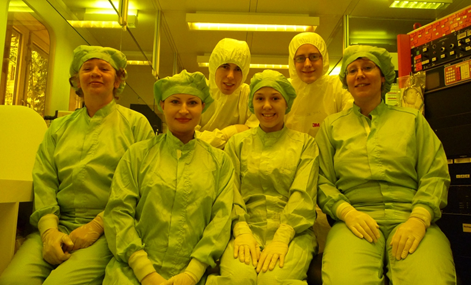
\includegraphics[scale=1, trim = 0cm 0cm 0cm 0cm,clip]
                	{./HerstellungBilder/Endbild.png}
                  \caption{geschafft!!!}
                \label{fig:geschafft}
            \end{figure}
            
    		\vspace{2em}
    		
    	\end{quote}
    		
\end{quote}
%--------------------------------------------------------------------
%--------------------------------------------------------------------

% \section{Kennlinie}
% \begin{quote}
%     
%     Benennung der Dateien:\\
%     Kennlinie_{Wavernummer}_Die_[{Zeile},{Spalte}]_Mess_{messung}.mat\\
%     
%     100 µA Strombegrenzung\\
%     Welche Diode?
%     Welcher Manipulator
%     
%     SMU1 = GNDi
%     SMU2 = GND
%     SMU3 = Var1
%     
%     Unterdiffusion
%     
%     unterspannung
%     0.0 & 2.4
%     0.5 & 3.8
%     0.8 & 4.5
%     1.0 & 5.0
%     1.3 & 5.5
%     1.8 & 6.7
%     2.5 & 8.2
%     3.0 & 9.2
%     
%     \TODO{müssen wir die Dies durchnummerieren?}
% \end{quote} %sec Kennlinie
% 
% %--------------------------------------------------------------------
% %--------------------------------------------------------------------
% 
% \section{Schaltverhalten}
% \begin{quote}
%     
%   
% 
% 
% 	In diesem Versuch soll Schaltverhalten bei Strom- und Spannungssprüngen 
% 	untersucht werden. Ein Maß für die Geschwindigkeit mit der die Diode 
% 	schalten kann ist die 
% 	Minoritätsträgerlebensdauer. Der Schaltvorgang hält 
% 	an, bis diese auf- bzw. abgebaut sind. Daher ist es Ziel dieses Versuches 
% 	über zwei unterschiedliche Verfahren diese Ladungsträgerlebensdauer zu 
% 	bestimmen. Dies ist zum einen der Stromausschaltvorgang und zum anderen die
%     Stromkommutierung.\\
% 
% 	Zunächst sollen das ideale und das reale Schaltverhalten gegenüber gestellt 
% 	werden. Das ideale Verhalten charakterisiert sich durch verzögerungs- und 
% 	verlustfreies Schalten. Die zu messenden Dioden zeigen allerdings durch 
% 	Energiespeicher wie die Sperrschicht- und die Diffusionskapazität kein 
% 	ideales Schaltverhalten. \\
% 
% 	Dabei ist die Charakteristik des Schaltverhaltens davon abhängig, ob es 
% 	sich um ein Spannungs- oder Stromsprung und einen Ein- oder Ausschaltvorgang 
% 	handelt. Um das Verständnis für diese Vorgänge zu verbessern, soll im 
% 	Folgenden näher auf einige Beispiele eingegangen werden.\\
% 
% 	Bei einem Einschaltstromsprung werden zwei Fälle unterschieden: Die starke 
% 	und die schwache Injektion. Ob starke oder schwache Injektion vorliegt 
% 	richtet sich nach der Ladungsträgeranzahl, die von der einen Seite des 
% 	pn-Überganges als Majoritätsträger auf die andere Seite als Minoritätsträger 
% 	gelangen. Ist die Anzahl der auf der anderen Seite ankommenden nun 
% 	Minoritäten in etwa so groß, oder größer wie die Majoritäten spricht man von
% 	starker Injekion. Andernfalls spricht man von schwacher Injektion.\\
%     Wie in Bild \ref{fig:Stromeinschalten} zu erkennen, spielt in den beiden 
%     Fällen der Bahnwiderstand eine unterschiedliche Rolle. Nach Shockley ist der 
%     Bahnspannungsabfall für schwache Injektion zu vernachlässigen. Mit Hilfe der 
%     Boltzmanfaktoren lässt sich ein logarthmischer Verlauf der Spannung über der 
%     RLZ herleiten. Dieser ist in der Abbildung \ref{fig:Stromeinschalten} in der 
%     grob gestrichelten Kennlinie zu erkennen. Man könnte vermuten, dass ohne den 
%     Bahnwiderstand nur der kapazitive Anteil zur Wirkung kommt und die Spannung
% 	daher kaum springen darf.\\
% 	Kommt hingegen der Einfluss des Bahnwiderstandes bei der starken Injektion 
% 	hinzu, dann kann ein heftiger
% 	Spannungssprung erfolgen. Der zusammengefasste Spannungsverlauf ist in Bild 
% 	\ref{fig:Stromeinschalten} an der durchgezogenen Kennlinie zu erkennen. 
% 	Durch den Bahnwiderstand bekommt die Diode vergleichbar mit Zuleitungen 
% 	einen induktiven Charakter und die Spannung kann springen.
% 
%     \begin{figure}[h]
%         \centering
%         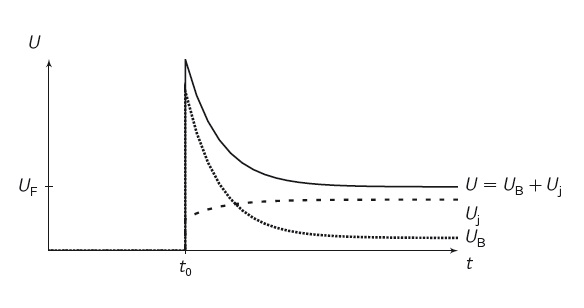
\includegraphics[scale=1]{Bilder/Stromeinschalten}
%         \caption{Spannungsverlauf beim Stromeinschaltsprung für starke und schwache Injektion \footnotemark}
%         \label{fig:Stromeinschalten}
%     \end{figure}
%          \footnotetext{Prof. Boit, Clemens Helfmeier, Philipp Scholz: Laborskript Technologie und Bauelemente der
% 	Halbleitertechnik (SS 2012), S. 78}
%    
%    \newpage
% 
%       \begin{table}[h]
%                \begin{addmargin}[-1cm]{3cm}
%                \centering
%                     \begin{tabular}{|p{5cm}|p{11.2cm}|}
%          \hline
%          Messung & Werte\\
%          \hline
%          Ausschaltvorgang & $I_{F}=10, 50, 100, 150 mA$\\
%    
%          \hline
%          Stromkommutierung & $I_{R0}=15,30,60,90,120 mA$\\
%          
%          \hline
%          
% 
%                     \end{tabular}
%                 \end{addmargin}
%              \caption{Messarten}
%           \label{Messarten}
%       \end{table}
%      
%       \vspace{2em}
% 
%       \begin{table}[h]
%      \begin{addmargin}[-1cm]{3cm}
%      \centering
%                      \begin{tabular}{|p{3cm}|p{3cm}|p{10.2cm}|}
%          \hline
%          Messung & Die/Diode/Wafer & gemessen\\
%          \hline
%          $R_{B} für I_{F}=10 mA$ & & \\
%                                  & & \\
%                                  & & \\
%                                  & & \\
%                                  & & \\
%                                  & & \\
%                                  & & \\
%                                  & & \\
%                                  & & \\
%                                  & & \\
%                                  & & \\
%                                  & & \\
%                                  & & \\
%          \hline
%          $R_{B} für I_{F}=50 mA$ & & \\
%                                  & & \\
%                                  & & \\
%                                  & & \\
%                                  & & \\
%                                  & & \\
%                                  & & \\
%                                  & & \\
%                                  & & \\
%                                  & & \\
%                                  & & \\
%                                  & & \\
%                                  & & \\
%          \hline
%          $R_{B} für I_{F}=100 mA$ & & \\
%                                  & & \\
%                                  & & \\
%                                  & & \\
%                                  & & \\
%                                  & & \\
%                                  & & \\
%                                  & & \\
%                                  & & \\
%                                  & & \\
%                                  & & \\
%                                  & & \\
%                                  & & \\
%          \hline
%          $R_{B} für I_{F}=150 mA$ & &\\
%                                  & & \\
%                                  & & \\
%                                  & & \\
%                                  & & \\
%                                  & & \\
%                                  & & \\
%                                  & & \\
%                                  & & \\
%                                  & & \\
%                                  & & \\
%                                  & & \\
%                                  & & \\
%    
%          \hline
% 
%                      \end{tabular}
%                  \end{addmargin}
%              \caption{Messwerte}
%            \label{Messwerte1}
%         \end{table}
%       
%        \vspace{2em}
%        
%        \begin{table}[h]
%      \begin{addmargin}[-1cm]{3cm}
%      \centering
%                       \begin{tabular}{|p{3cm}|p{3cm}|p{10.2cm}|}
%          \hline
%          Messung & Die/Diode/Wafer & gemessen\\
%          \hline
%          $\tau für I_{F}=150 mA$ & & \\
%                                  & & \\
%                                  & & \\
%                                  & & \\
%                                  & & \\
%                                  & & \\
%                                  & & \\
%                                  & & \\
%                                  & & \\
%                                  & & \\
%                                  & & \\
%                                  & & \\
%                                  & & \\
%          \hline
%          $t_{s}$ & & \\
%                                  & & \\
%                                  & & \\
%                                  & & \\
%                                  & & \\
%                                  & & \\
%                                  & & \\
%                                  & & \\
%                                  & & \\
%                                  & & \\
%                                  & & \\
%                                  & & \\
%                                  & & \\
%          \hline
%          $Q_{s}$ & &\\
%                                  & & \\
%                                  & & \\
%                                  & & \\
%                                  & & \\
%                                  & & \\
%                                  & & \\
%                                  & & \\
%                                  & & \\
%                                  & & \\
%                                  & & \\
%                                  & & \\
%                                  & & \\
%          \hline
%          $\tau$ & &\\
%                                  & & \\
%                                  & & \\
%                                  & & \\
%                                  & & \\
%                                  & & \\
%                                  & & \\
%                                  & & \\
%                                  & & \\
%                                  & & \\
%                                  & & \\
%                                  & & \\
%                                  & & \\
%          \hline
% 
%                            \end{tabular}
%                     \end{addmargin}
%              \caption{Messwerte}
%          \label{Messwerte2}
%       \end{table}
%       
%       \vspace{2em}
%       
%       \begin{table}[h]
%                  \begin{addmargin}[-1cm]{3cm}
%      \centering
%                      \begin{tabular}{|p{3cm}|p{3cm}|p{10.2cm}|}
%          \hline
%          Messung & Die/Diode/Wafer & gemessen\\
%          \hline
%          Tempertatur & & \\
%                                  & & \\
%                                  & & \\
%                                  & & \\
%                                  & & \\
%                                  & & \\
%                                  & & \\
%                                  & & \\
%                                  & & \\
%                                  & & \\
%                                  & & \\
%                                  & & \\
%                                  & & \\
%          \hline
%          Vorwärtsstrom & & \\
%                                  & & \\
%                                  & & \\
%                                  & & \\
%                                  & & \\
%                                  & & \\
%                                  & & \\
%                                  & & \\
%                                  & & \\
%                                  & & \\
%                                  & & \\
%                                  & & \\
%                                  & & \\
%          \hline
%          Rückwärtsstrom & &\\
%                                  & & \\
%                                  & & \\
%                                  & & \\
%                                  & & \\
%                                  & & \\
%                                  & & \\
%                                  & & \\
%                                  & & \\
%                                  & & \\
%                                  & & \\
%                                  & & \\
%                                  & & \\
%          \hline
%                      \end{tabular}
%                   \end{addmargin}
%              \caption{Sonstige Angaben zur Messung}
%          \label{AngabenZurMessung}
%       \end{table}
%       
%       \noindent
%       
%        \vspace{2em}
%       
% \end{quote} %sec Schaltverhalten
% 
% 
% 
% \begin{thebibliography}{999}
% 
% % \bibitem{Boris}Boris Henckell: Ein Paar sachen geklaut.. ähhh inspirationen geholt
% % \href{http://www.krachler.com/fileadmin/user_upload/arbeiten/Reglersynthese_Christian_Krachler.pdf}{Reglersynthese nach dem Frequenzkennlinienverfahren}, S16, S22, 08.05.2012
% 
% 
% % Name, Vorname.; evtl. Name2, Vorname2.: Titel des Dokumentes
% % oder Buches, Zeitschrift/Verlag/URL (Auflage, Erscheinungsort, -jahr), ggf. Seitenzahlen
% %\bibitem [Wiki10] {DigitaleMesskette2} \url{www.wikipedia.org}, Zugriff 22.03.2010
% 
% \bibitem [1]{TBH} Prof. Boit, Clemens Helfmeier, Philipp Scholz: Laborskript Technologie und Bauelemente der
% Halbleitertechnik (SS 2012)
% \end{thebibliography}
%     
% \end{quote} %sec Schaltverhalten
% 
% %--------------------------------------------------------------------
% %--------------------------------------------------------------------
% 
% \section{Emissionsmessung}
% \begin{quote}
%     
%     Eine Emissionsmessung ist in der Halbleitertechnologie insofern interessant,
%     weil sie Erkenntnisse über charakteristische Eigenschaften des Halbleiters,
%     in unserem Fall die selbst hergestellte Diode, liefert. Dazu gehören die
%     Ladungsträgerlebensdauer $\tau_{n,p}$ und die Diffusionslänge $L_{n,p}$. Auf
%     die Lebensdauer lässt sich mithilfe der Diffusionslänge und des
%     Diffusionskoeffizienten schließen. Dieser ist ein materialabhängiger Wert,
%     welcher von uns nicht weiter beachtet wird. Der folgende Zusammenhang hilft
%     bei der Berechnung von $\tau_{n,p}$:
%     
%     \begin{equation*}
%         \begin{split}
%             L_{n,p} = \sqrt{\tau_{n,p} \cdot D_{n,p}} 
%         \end{split}
%     \end{equation*}
%     
%     Ziel unserer Messung aber war die Bestimmung der Diffusionslänge in unserer
%     Diode. Dieser wurde über die realisierte Intensitätsmessung anhand der
%     Emissionen in der Diode ermittelt. Dabei wurden folgende
%     Proportionalitätsverhätnisse verwendet:
%     
%     \begin{equation*}
%         \begin{split}
%             I(x) \sim \ \Delta n \sim \ exp(-\frac{x}{L_n}) 
%         \end{split}
%     \end{equation*}
%     
%     Hierbei werden Strahlungsintensität ins Verhältnis mit der\\
%     Minoritätsüberschussladungträgerkonzentration und dieser wiederum 
%     ins Verhältnis mit einem Exponentialtherm gesetzt. Daher kann man die
%     Intensitätsmessung direkt mit diesem Therm in Verbindung setzen, 
%     welcher in seinem Argument die gesuchte Diffusionslänge beinhaltet. Weiteres
%     zur Berechnung des $L_n$ steht in der Auswertung der Messung.\\
%     
%     Um aber die Intensitätsmessung verstehen zu können müssen einige
%     grundlegende Theorien der Halbleiter bezüglich ihrer Typen und ihrer
%     Rekombinationsarten behandelt und nachvollzogen werden.\\ 
%     Daher gibt es vor der Versuchsdurchführung und der Auswertung zunächst eine
%     kleine Exkursion in den theoretischen Bereich.
%     
%         \subsection{Direkter und indirekter Halbleiter }
%         \begin{quote}
%         
%         Es gibt zwei Arten von Halbleitern, die direkten und die indirekten
%         Halbleiter. Diese unterscheiden sich darin, dass die Rekombination eines
%         Ladungsträgers aus dem Leitungs- in das Valenzband unterschiedliche
%         Vorraussetzungen erfordert.
%             
%             \subsubsection{direkter Halbleiter}
%             \begin{quote}
%             Die Rekombination bei einem direkten Halbleiter ist relativ simpel.
%             Ein freies Elektron braucht dabei nur, unter Abgabe der jeweiligen
%             Energie, den Bandabstand zwischen Leitungs- und Valenzband zu
%             überqueren.
%             
%             \begin{figure}[H]
%                     \centering
%                         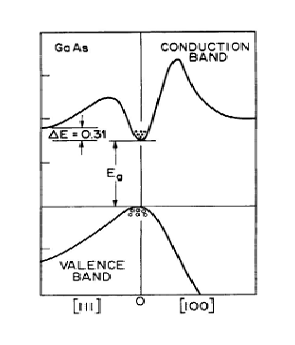
\includegraphics[scale=0.72, trim = 1cm 0cm 1.5cm 0cm,
%                         clip]{./Emissionsbilder/restliches/direkt.png}
%                         \caption{Rekombination bei einem direkten Halbleiter}
%                             \label{fig:./Emissionsbilder/restliches/direkt.png}
%             \end{figure}
%             
%             
%             \end{quote}       
%         
%             \subsubsection{indirekter Halbleiter}
%             \begin{quote}
%             Die Rekombination bei einem indirekten Halbleiter erfordert neben
%             einem Energieunterschied auch einen Impulsunterschied, damit das
%             Elektron auf dem Valenzband auftreffen kann. Dieser
%             Impulsunterschied ist in der folgenden Abbildung zu erkennen.
%             
%             \begin{figure}[H]
%                     \centering
%                         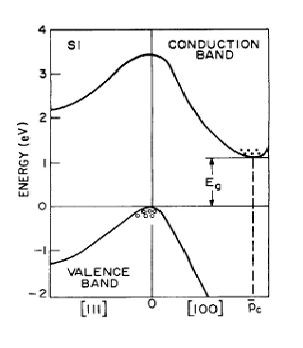
\includegraphics[scale=0.73, trim = 1cm 0cm 1.5cm 0cm,
%                         clip]{./Emissionsbilder/restliches/indirekt.png}
%                         \caption{Rekombination bei einem indirekten Halbleiter}
%                             \label{fig:./Emissionsbilder/restliches/indirekt.png}
%             \end{figure}
%             
%             \TODO{Bildquellen, TBH-Skript S.92 einfügen}
%             \end{quote}       
%             
%             Ein weiterer Unterschied zwischen direkten und indirekten
%             Halbleitern ist der, dass direkte Halbleiter hauptsächlich
%             strahlend rekombinieren, wohingegen indirekte Halbleiter
%             stochastisch betrachtet fast nur nichtstrahlend rekombinieren.
%             Dennoch findet mit sehr geringer Wahrscheinlichkeit auch vereinzelt
%             strahlende Rekombination in den indirekten Halbleitern statt.\\
%             Bevor weiter darauf eingegangen wird, in wie fern dies für die
%             Emissionsmessung von Bedeutung ist, werden die Rekombinationsarten,
%             strahlend und nichtstrahlend, wiederholt.
%             
%         \end{quote}
%         
%         \subsection{Rekombinationsmechanismen}
%         \begin{quote}
%         
%         Eine Rekombination erfolgt stets unter Abgabe von einer
%         Energiedifferenz. Dabei wird unterschieden, ob diese Energie in Form
%         eines Lichtquants oder von Wärme abgegeben wird, wodurch auch die
%         Beschreibung strahlend oder nichtstrahlend entsteht.\\
%         Nun folgen je ein Beispiel für diese Machanismen.
%         
%             \subsubsection{strahlende Rekombination}
%             \begin{quote}
%             
%             Die strahlende Rekombination, hauptsächlich bei direkten Halbleitern
%             zu sehen, besagt, dass der rekombinierende Ladungsträger die
%             Energiedifferenz, welche er zurücklegt, in Form eines Photons
%             freigibt. Die Energie dieses Photons beträgt genau die Energie des
%             Bandabstands zwischen den beiden Bändern. Anders ausgedrückt kann
%             man sie auch Rekombinationsenergie nennen:
%                     
%             \begin{equation*}
%                 \begin{split}
%                     W_{Rek} = h \cdot \nu 
%                 \end{split}
%             \end{equation*}
%             
%             Diese Rekombinationsenergie setzt sich aus des Produkt aus dem
%             Planckschen Wirkungsquantums $h$ und die Frequenz des entstehenden
%             Lichts $\nu$.\\
%             
%             Ein Beispiel für die strahlende Rekombination ist die
%             Band-Band-Rekombination, welche in der folgenden Abbildung
%             dargestellt wurde:
%             
%             \begin{figure}[H]
%                     \centering
%                         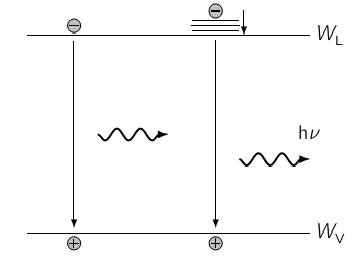
\includegraphics[scale=0.68, trim = 1cm 0cm 1.5cm 0cm,
%                         clip]{./Emissionsbilder/restliches/bandband.png}
%                         \caption{strahlende Band-Band-Rekombination}
%                             \label{fig:./Emissionsbilder/restliches/direkt.png}
%             \end{figure}
%             
%             Man erkennt ein Elektron, welches beim Rekombinieren, die bereits
%             erwähnte Rekombinationsernergie in Form eines Photons abgibt. Es
%             kann aber auch vorkommen, dass die abgegebene Energie an ein
%             weiteres Eektron im Leitungsband abgegeben wird, wodurch dieser auf
%             ein höheres Energieniveau im Leitungsband angehoben und wieder runterfallen 
%             kann. Diese Möglichkeit ist bei der strahlenden Rekombination die
%             unwarscheinlichere Variante.
%             
%             \end{quote}
%             
%             \subsubsection{nichtstrahlende Rekombination}
%             \begin{quote}
%             
%             Die nichtstrahlende Rekombination findet hauptsächlich bei
%             indirekten Halbleitern statt. Dabei wird die Rekombinationsenergie
%             an ein weiteres Elektron im Leitungsband abgegeben, welches auf ein
%             höheres Energieniveau angehoben wird und unter Abgabe von
%             thermischer Energie wieder runterfallen kann.\\
%             Als ein Beispiel für die nichtstrahlende Rekombination wird die
%             Augerrekombination dargestellt:
%             
%             \begin{figure}[H]
%                     \centering
%                         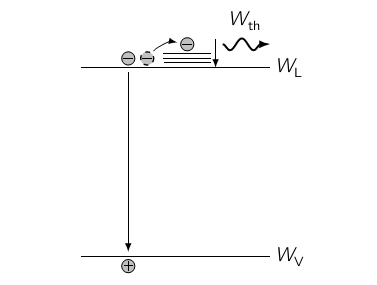
\includegraphics[scale=0.78, trim = 1cm 0cm 1.5cm 0cm,
%                         clip]{./Emissionsbilder/restliches/auger.png}
%                         \caption{nichtstrahlende Auger-Rekombination}
%                             \label{fig:./Emissionsbilder/restliches/auger.png}
%             \end{figure}
%             
%             \TODO{Bildquellen einfügen: TBH-Skript S.93,94}
%             \end{quote}
%         
%         Die für die Emissiosmessung verwendete Diode besteht aus Silizium,
%         welcher ein indirekter Halbleiter ist und dessen Rekombinationen
%         hauptsächlch nichtstrahlend sind. Wie aber schon bei den Halbleitertypen
%         erwähnt, kann es bei indirekten Halbleitern auch mit sehr geringer
%         Wahrscheinlichkeit zu strahlender Rekombination kommen. Da die Abgabe
%         von thermischer Energie zu einem Temperaturunterschied in der Diode
%         führen würde, bräuchte man bei den Emissionsmessung sehr feine und genau
%         Thermometer, welche im $\mu m$-Bereich nicht realisierbar sind. Daher
%         wird die stochastisch in geringer Menge vorhandene strahlende
%         Rekombination betrachtet um über die mit lichtempfindlichen
%         Kameras gemessene Lichtintensitäten auf die gesuchte Diffusionslänge
%         schließen zu können.
%         
%         \end{quote}
%         
%         \vspace{1.5em}
%         
%         Emission entsteht bei der Rekombination eines freien Ladungsträgers,
%         welches nur in Durchlassrichtung bei einer Diode erwartet wird. Dabei
%         werden die Majoritäten ins entgegen gesetztes Gebiet injeziert und
%         rekombinieren dort als Minoritäten mit den oppositär gepolten
%         Ladungsträgern. Die dabei freigesetzte Energie kann dann als Emission
%         wargenommen werden. Emission kann aber auch in Sperrrichtung entstehen.
%         Die sogennante Feldemission findet dabei ausschließlich in der
%         ausgebreiteten Raumladungszone statt. Sobald eine Sperrspannung an der
%         Diode angelegt wird, werden die freien Ladungsträger aus der
%         Raumladungszone gesaugt und erfahren dabei eine kinetische Energie,
%         dessen Stärke von der Größe der Sperrspannung abhängt. Während der
%         beschleunigten Bewegung der Ladungsträger aus der Raumladungszone,
%         können diese mit Gitteratomen zusammenprallen und Elektronen aus diesem
%         Atom auf ein höheres Energieniveau anheben. Wie bei der nichtstrahlenden
%         Rekombination entsteht bei diesem Vorfall hauptsächlich thermische
%         Energie,es kann aber auch, mit einer sehr kleinen wahrscheinlichkeit
%         eine strahlende Rekombination vorkommen.\\
%         Die Feldemission ist im Vergleich zu der Emission in Flussrichtung
%         unbedeutend klein. Daher ist für die Intensitätsmessung nur eine
%         Emission in Flussrichtung relevant.
%         
%         \vspace{1.5em}
%         
%         \subsection{Messaufbau}
%         \begin{quote}
%         
%         Die Emissionsmessung erfolgt, wie in der Einleitung erwähnt, durch eine
%         Intensitätsmessung während der Rekombinationen in Flussrichtung der
%         Diode. Die Messung wird mithilfe des Phemos 1000 durchgeführt, welches
%         ein Prüfgerät in der Halbleitertechnik ist und hauptsächlich für
%         Fehlerdetektion dient. Um diese geringe Lichtintensität
%         messen zu können, braucht man eine lichtempfindliche CCD Kamera. Diese
%         ist im Phemos integriert und muss während der gesamten Messung auf
%         $-50$°C gekühlt werden. So werden thermische Rauscheinflüsse der sehr 
%         empfindlichen Kamera vermieden um das Ergebnis nicht zu verfälschen.\\
%         
%         Der Wafer, mit mehreren Diodenstrukturen, wird in dem Innenraum des
%         Phemos auf einer Vakuumplatte fixiert, sodass der erwünschte Bereich des
%         Wafers mit dem passenden Objektiv vergrössert werden kann. Diese
%         Vergrößerung hilft bei der Kontaktierung des p- und des n-Pads der Diode
%         anhand Nadelspitzen, welche in der unteren Abbildung im Licht des
%         Mikroskops zu erkennen sind.
%         
%         \begin{center}
%                 \begin{tabular}{ll}
%     
%                 \hspace{-8em}
%                     \begin{minipage}{0.6\textwidth}
%     
%                         \begin{figure}[H]
%                             \label{fig:}
%                             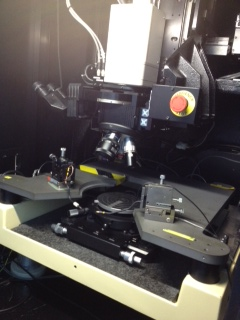
\includegraphics[scale=0.7, trim = 0cm 0cm 0cm
%                             0cm, clip]{./Emissionsbilder/restliches/phemos1.JPG}
%                             %FIXME [width=640px,
%                              %height=474px]
%                             \caption{Innenraum des Phemos}
%                         \end{figure}
%     
%                     \end{minipage}
%                     \begin{minipage}{0.6\textwidth}
%     
%                         \begin{figure}[H]
%                             \label{fig:}
%                             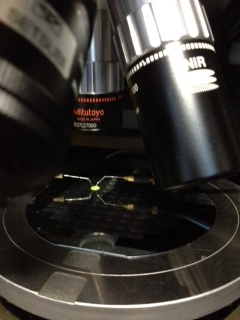
\includegraphics[scale=0.7, trim = 0cm 0cm 0cm
%                             0cm, clip]{./Emissionsbilder/restliches/phemos2.JPG}
%                             %FIXME [width=640px,
%                              %height=474px]
%                             \caption{kontaktierte Diode auf dem Wafer}
%                         \end{figure}
%                     \vspace{-1.5em}
%     
%                     \end{minipage}
%     
%                 \end{tabular}
%                 \end{center}
%         
%         \vspace{2em}
%         
%         Anhand eines Live-Bilds der CCD Kamera, kann man bis zum Start der
%         Messung den fokussierten Bereich bepannungsquelle für den
%         Durchlassbetrieb der Diode wurde der HP4145A, ein sensibeles
%         Analysegerät für Halbleiterbauelemente, verwendet, mit welchem eine
%         konstante Spannung für eine einstellbare Zeitspanne eingestellt werden
%         kann. Somit konnte man fest davon ausgehen, dass die Diode ohne einen
%         Spannungseinbruch konstant in Durchlassrichtung betrieben wurde.\\
%         Die Messdauer der Emission wurde mithilfe der Phemos-Software
%         eingestellt. Mit welchen Durchlassspannungen und wie lange gemessen
%         wurde, wird in der Auswertung der Messergebnisse angegeben.
%         
%         \vspace{1em}
%         
%         Am Ende jeder Messung wurde noch eine Dark-Substraction durchgeführt.
%         Bei dieser Dark-Substraction wird die Durchlassspannung abgeschaltet,
%         wodurch die Diode nicht mehr als aktiv betrachtet wird. Die Emissionsmessung wird mit der
%         gleichen Messdauer und deaktivierter Diode nochmal durchgeführt und von
%         der eigentlichen Emissionsmessung subtrahiert, damit jegliche
%         Rauscheinflüsse des Phemos selbst aus den Messergebnissen ausgeschlossen
%         werden können. 
%         
%         \end{quote}
%         
%         \subsection{Messergebnisse}
%         \begin{quote}
%         
%         Die Active-Area- und Kontaktfenstermasken wurden so erstellt, dass der
%         Wafer am Ende der Produktion Dioden auf jedem Die besaß, die für diese
%         Emissionsmessung hergestellt wurden. Diese Emissions-Dioden haben die
%         Besonderheit, dass zwischen p- und n-Pad das Substrat nicht mit Siliziumoxid beschichtet
%         ist, damit an den pn-Übergang zwischen n-Gebiet und p-Substrat
%         unverfälschte Emission gemessen werden kann.\\ 
%         Man hätte annehmen können, dass dort, wo Oxid auf dem pn-Übergang lag,
%         keine Emission aus dem Wafer austreten und gemessen werden kann. Die Praxis bewies aber das
%         Gegenteil. Unabhängig von der Auswertung der Messung
%         konnte an den pn-Übergängen mit Siliziumoxid darüber eine viel stärkere
%         Emission gemessen werden. Der Grund dafür liegt in dem Brechungsindex
%         und der Dicke der Oxidschicht, denn durch die Reflexionen der Strahlung an
%         den Übergängen von Silizium zu Siliziumoxid und Siliziumoxid zur Luft
%         werden die Strahlen so reflektiert, dass konstruktive Interferenz
%         zwischen den Lichtwellen entsteht und somit die Emission als viel
%         stärker wahrgenommen wird. Da dies nicht die wirkliche Intensität der
%         Emission am pn-Übergang unserer Diode wiederspiegelt, wurden diese mit
%         Oxid überlagerten Stellen in der Emissionsmessung vernachlässigt.\\
%         
%         Gemessen wurde nur der Bereich von der Grenze des n-Gebiets bis in
%         das p-Substrat hinein. Als Hilfe dafür wurde das jeweilige Emissionsbild
%         der Phemos-Software verwendet. Diese zeigte mit farblichen Unterschieden
%         (rot = starke Emission, blau = schwache Emission) wo der sinnvolle
%         Messbereich begann und endete. Die folgenden Abbildungen zeigen die
%         Diode vor und nach der Emissionsmessung auf dem Die in Zeile $6$ und
%         Spalte $3$ des Wafers. Zunächst wurde eine große, dann eine kleinere
%         Emissions-Diode ausgemessen. Bei beiden betrug die Durchlassspannung
%         $1,2\ V$ bei $25\ mA$ und einer Messdauer von $4s$.
%         
%          \begin{center}
%                 \begin{tabular}{ll}
%     
%                 \hspace{-10em}
%                     \begin{minipage}{0.6\textwidth}
%     
%                         \begin{figure}[H]
%                             \label{fig:}
%                             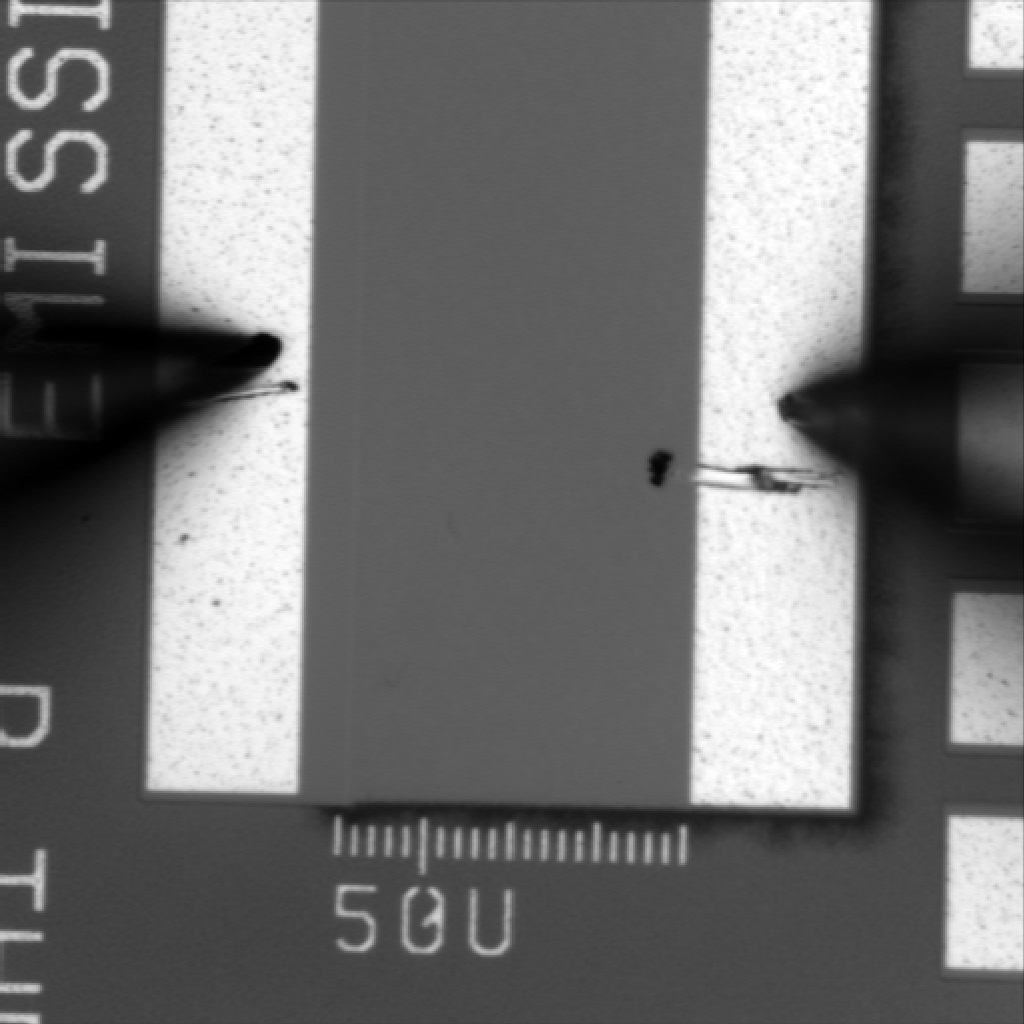
\includegraphics[scale=0.25, trim = 0cm 0cm 0cm
%                             0cm,
%                             clip]{./Emissionsbilder/eins/nach_Kontaktierung_vorMessung.jpg}
%                             %FIXME [width=640px, height=474px]
%                             \caption{kontaktierte Diode, Live-Bild der CCD
%                             Kamera}
%                         \end{figure}
%     
%                     \end{minipage}
%                     \begin{minipage}{0.6\textwidth}
%     
%                          \begin{figure}[H]
%                             \label{fig:}
%                             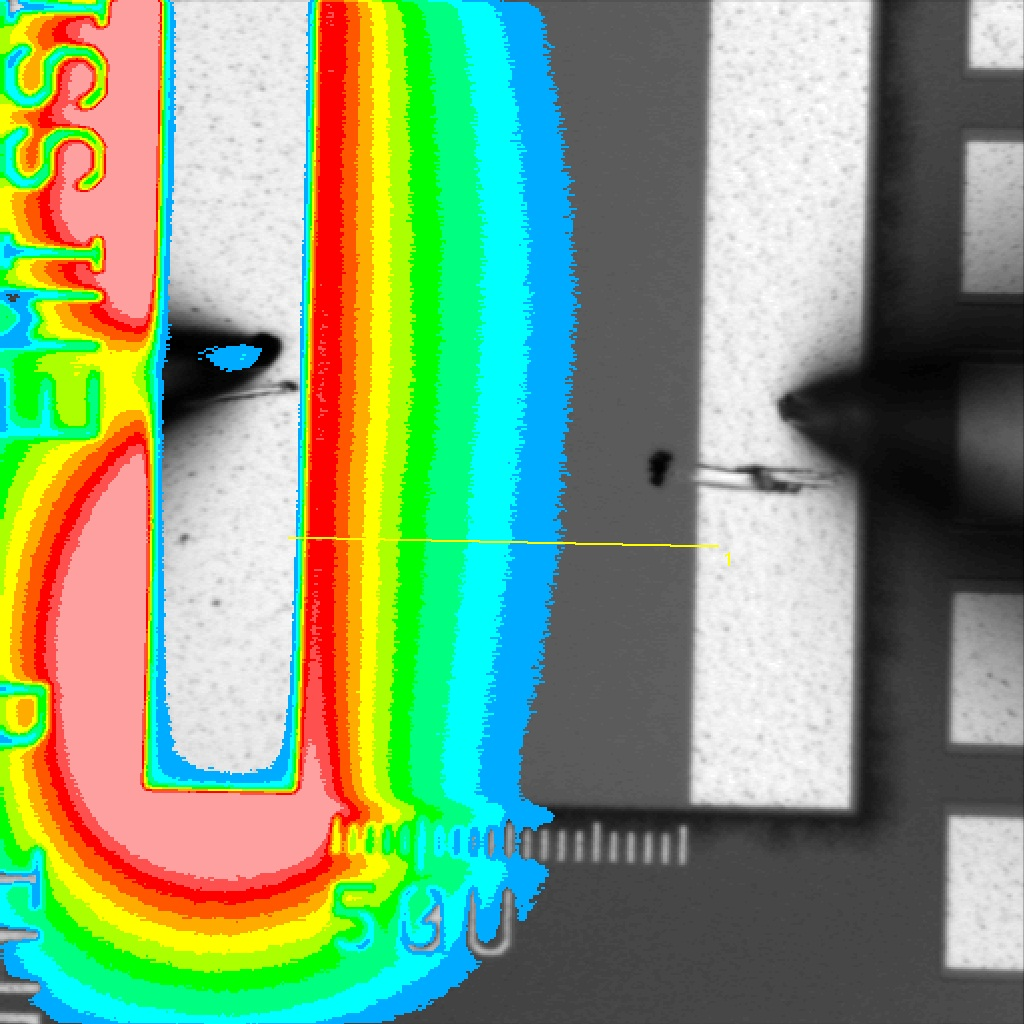
\includegraphics[scale=0.25, trim = 0cm 0cm 0cm
%                             0cm,
%                             clip]{./Emissionsbilder/eins/nach_Emission_mit_Distanzen.jpg}
%                             %FIXME [width=640px, height=474px]
%                             \caption{selbe Diode nach der Emissionsmessung}
%                         \end{figure}
%                    \vspace{-1.5em}
%     
%                     \end{minipage}
%     
%                 \end{tabular}
%                 \end{center}
%                 
%         \vspace{2em}
%         
%         Der gelbe Strich wurde anhand der Maus gezogen und zeigt den Bereich im
%         Substrat, welcher genauer ausgewertet wurde. Mehr dazu folgt in der
%         Auswertung.\\
%         
%         Als nächstes folgen die Abbildungen der kleineren Emissions-Diode auf
%         dem selben Die:
%              
%         
%          \begin{center}
%                 \begin{tabular}{ll}
%     
%                 \hspace{-10em}
%                     \begin{minipage}{0.6\textwidth}
%     
%                         \begin{figure}[H]
%                             \label{fig:}
%                             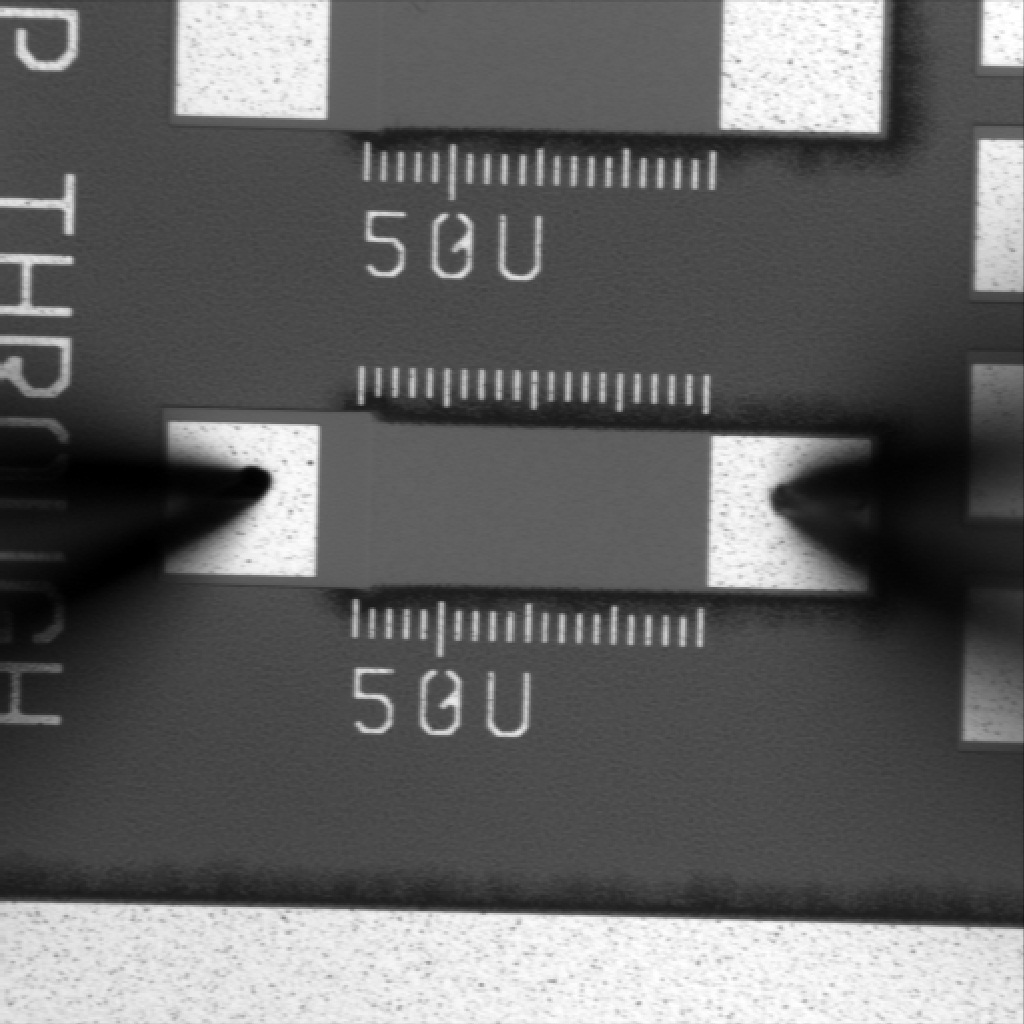
\includegraphics[scale=0.25, trim = 0cm 0cm 0cm
%                             0cm,
%                             clip]{./Emissionsbilder/zwei/nack_Kontaktierung.jpg}
%                             %FIXME [width=640px, height=474px]
%                             \caption{kontaktierte Diode, Live-Bild der CCD
%                             Kamera}
%                         \end{figure}
%     
%                     \end{minipage}
%                     \begin{minipage}{0.6\textwidth}
%     
%                          \begin{figure}[H]
%                             \label{fig:}
%                             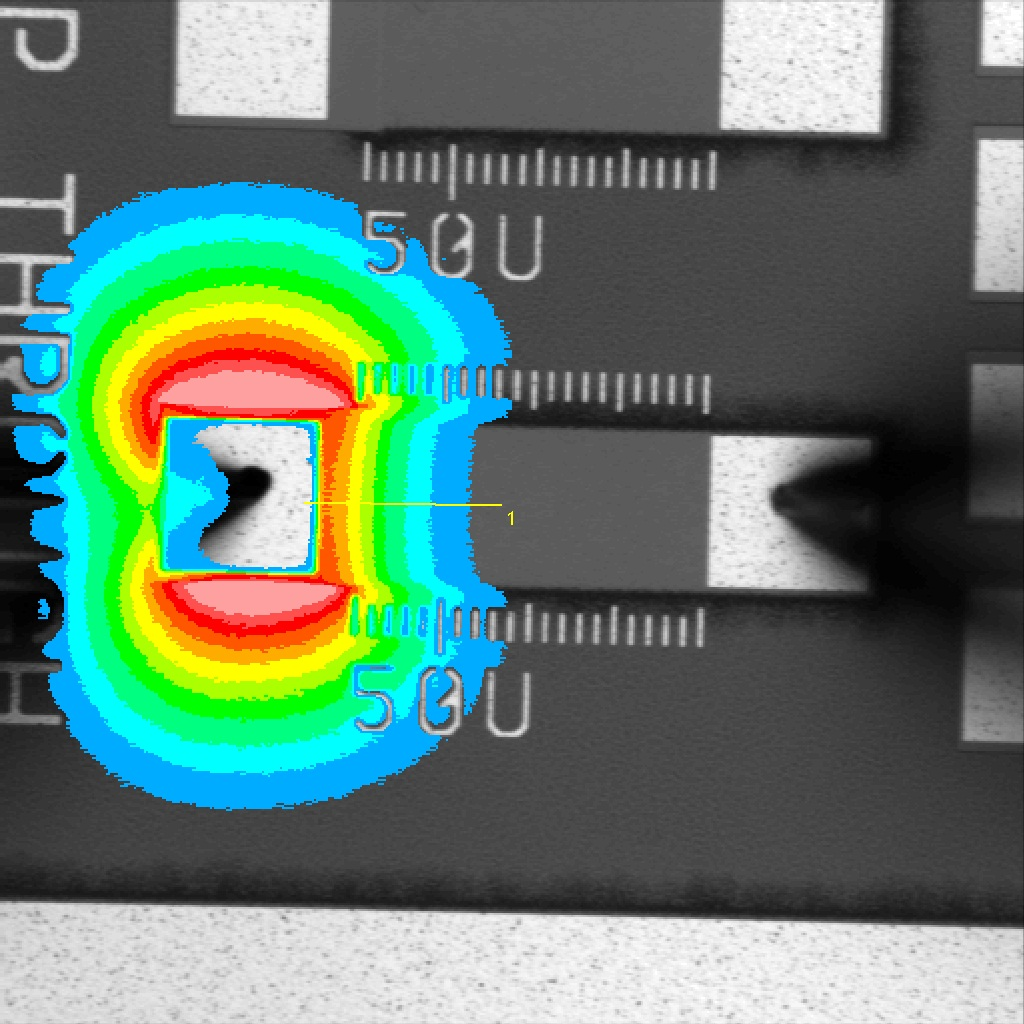
\includegraphics[scale=0.25, trim = 0cm 0cm 0cm
%                             0cm,
%                             clip]{./Emissionsbilder/zwei/nach_Emissionsmessung_Intensitat_Distanz.jpg}
%                             %FIXME [width=640px, height=474px]
%                             \caption{selbe Diode nach der Emissionsmessung}
%                         \end{figure}
%                    \vspace{-1.5em}
%     
%                     \end{minipage}
%     
%                 \end{tabular}
%                 \end{center}
%                 
%         \vspace{2em}
%         
%         Nun wurde noch ein Die am Rand des Wafers ausgemessen um nach
%         Unterschieden zwischen den Messergebnissen kontrolliert werden zu
%         können. Auch auf dem Die in Zeile $15$ und Spalte $8$ wurde erst eine
%         große, dann eine kleine Emissions-Diode untersucht. Die Durchlassspannung bei der
%         großen Diode betrug $1,2\ V$ bei einem Strom von $25\ mA$. Die Messdauer
%         wurde aus $3s$ variiert.
%         
%         
%          \begin{center}
%                 \begin{tabular}{ll}
%     
%                 \hspace{-10em}
%                     \begin{minipage}{0.6\textwidth}
%     
%                         \begin{figure}[H]
%                             \label{fig:}
%                             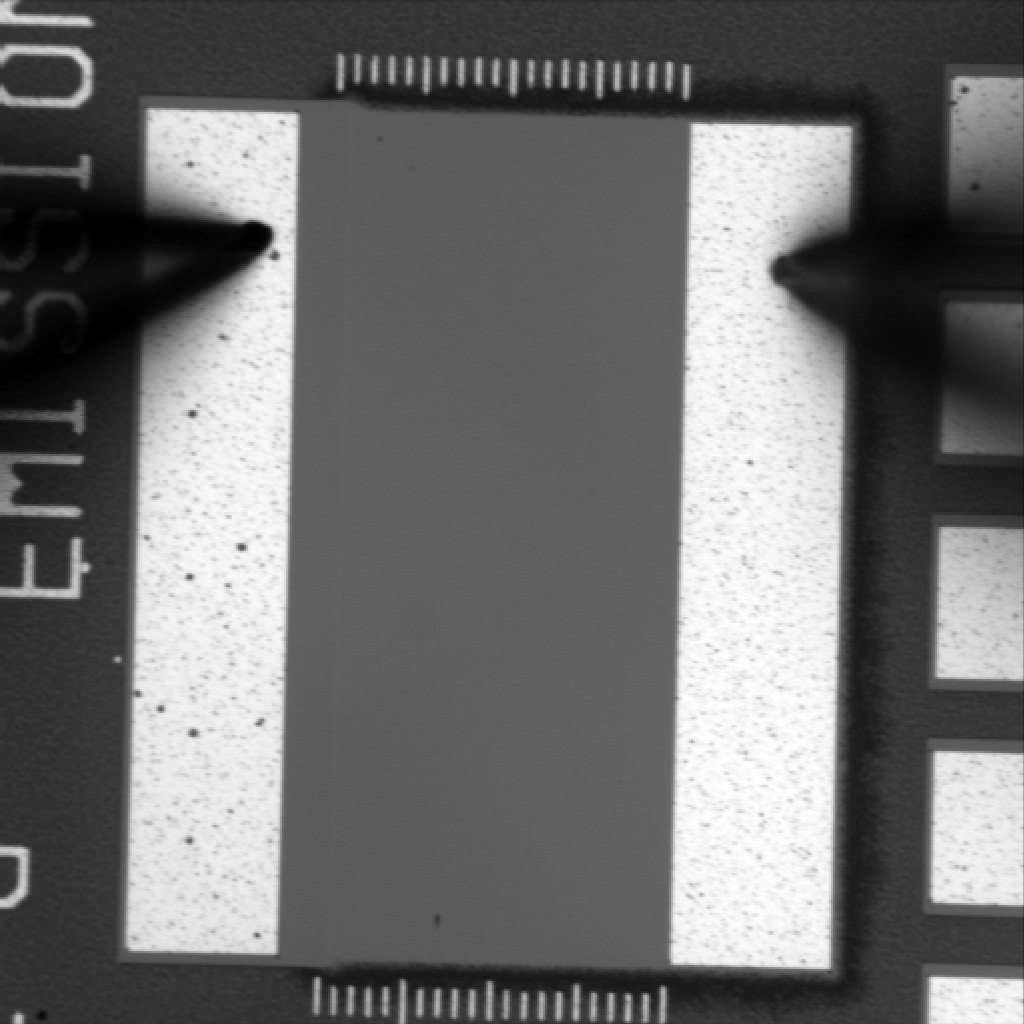
\includegraphics[scale=0.25, trim = 0cm 0cm 0cm
%                             0cm,
%                             clip]{./Emissionsbilder/drei/nach_Kontaktierung.jpg}
%                             %FIXME [width=640px, height=474px]
%                             \caption{kontaktierte Diode, Live-Bild der CCD
%                             Kamera}
%                         \end{figure}
%     
%                     \end{minipage}
%                     \begin{minipage}{0.6\textwidth}
%     
%                          \begin{figure}[H]
%                             \label{fig:}
%                             \includegraphics[scale=0.25, trim = 0cm 0cm 0cm
%                             0cm,
%                             clip]{./Emissionsbilder/drei/nach_Emissionsmessung_Distanz.jpg}
%                             %FIXME [width=640px, height=474px]
%                             \caption{selbe Diode nach der Emissionsmessung}
%                         \end{figure}
%                    \vspace{-1.5em}
%     
%                     \end{minipage}
%     
%                 \end{tabular}
%                 \end{center}
%                 
%         \vspace{2em}
%         
%         Die Durchlassspannung der kleineren Diode betrug $1,5\ V$ bei $30\ mA$
%         Strom. Die Messdauer wurde auf $4s$ gestellt. Vor und nach der Messung
%         wurden folgende Bilder aufgezeichnet:
%         
%          
%          \begin{center}
%                 \begin{tabular}{ll}
%     
%                 \hspace{-10em}
%                     \begin{minipage}{0.6\textwidth}
%     
%                         \begin{figure}[H]
%                             \label{fig:}
%                             \includegraphics[scale=0.25, trim = 0cm 0cm 0cm
%                             0cm,
%                             clip]{./Emissionsbilder/vier/nach_Kontaktierung.jpg}
%                             %FIXME [width=640px, height=474px]
%                             \caption{kontaktierte Diode, Live-Bild der CCD
%                             Kamera}
%                         \end{figure}
%     
%                     \end{minipage}
%                     \begin{minipage}{0.6\textwidth}
%     
%                          \begin{figure}[H]
%                             \label{fig:}
%                             \includegraphics[scale=0.25, trim = 0cm 0cm 0cm
%                             0cm,
%                             clip]{./Emissionsbilder/vier/nach_Emission_Distanz.jpg}
%                             %FIXME [width=640px, height=474px]
%                             \caption{selbe Diode nach der Emissionsmessung}
%                         \end{figure}
%                    \vspace{-1.5em}
%     
%                     \end{minipage}
%     
%                 \end{tabular}
%                 \end{center}
%                 
%         \vspace{2em}
%         
%         Bislang ist nur eine Emissionsintensität zu sehen. Mithilfe der
%         Phemos-Software konnte daraus ein Intensitätsprofil erstellt werden,
%         woraus am Ende dann auf die Diffusionslänge zurück geschlossen werden
%         kann.
%         
%         \vspace{1.5em}
%         
%         Es wurde auch eine Fingerstrukter-Diode für die Messung verwendet,
%         welche sich ebenfalls auf dem äußeren Die befand. Eine
%         Diffusionslängenberechnung wurde für diese Diode nicht durchgeführt, da
%         am Phemos ein Objektiv gewählt wurde, mit der die gesamte Diode auf des
%         Bildschirm sichtbar war. Daher sind die Fingerstrukturen zwar sichtbar,
%         aber die pn-Übergänge zwischen n-Finger und dem p-Substrat dazwischen,
%         die Grenze an der die Emission erwartet wird, sind viel zu klein
%         abgebildet, als dass eine Intensitätskurve mit der geringen Vergrößerung
%         sinnvoll wäre. Daher sind nur die Kontaktierung und das Ergebniss der
%         Emissionsmessung im Protokoll aufgeführt. Die Durchlassspannung während
%         der Messung betrug $5\ V$ bei einem Strom von $20\ mA$ und einer
%         Messdauer von $4s$. 
%         
%         
%             \begin{center}
%                 \begin{tabular}{ll}
%     
%                 \hspace{-10em}
%                     \begin{minipage}{0.6\textwidth}
%     
%                         \begin{figure}[H]
%                             \label{fig:}
%                             \includegraphics[scale=0.25, trim = 0cm 0cm 0cm
%                             0cm,
%                             clip]{./Emissionsbilder/fuenf/nach_Kontaktierung.jpg}
%                             %FIXME [width=640px, height=474px]
%                             \caption{kontaktierte Diode, Live-Bild der CCD
%                             Kamera}
%                         \end{figure}
%     
%                     \end{minipage}
%                     \begin{minipage}{0.6\textwidth}
%     
%                          \begin{figure}[H]
%                             \label{fig:}
%                             \includegraphics[scale=0.25, trim = 0cm 0cm 0cm
%                             0cm,
%                             clip]{./Emissionsbilder/fuenf/SuperImpose.jpg}
%                             %FIXME [width=640px, height=474px]
%                             \caption{selbe Diode nach der Emissionsmessung}
%                         \end{figure}
%                    \vspace{-1.5em}
%     
%                     \end{minipage}
%     
%                 \end{tabular}
%                 \end{center}
%                 
%         \vspace{2em}
%         
%         Man kann erkennen, dass die n-Finger, welche von links nach rechts
%         Richtung p-Pad reichen, die Positionen der pn-Übergänge bilden. Daher
%         wäre eigentlich eine Emission entlang der Ränder der n-Finger zu erwarten.
%         Eine Erklärung, warum aber die größte Emission nur an der Stelle
%         auftritt, wo der Abstand zwischen n- und p-Pad am geringsten ist, wäre, dass die
%         Rekombination hinter der Raumladungszone dort viel größer ist, wo der
%         Halbleiter den geringsten Widerstand aufweist. Der Strom könnte also
%         dort am größten werden, wodurch eine stärkere Emission erklärt wäre.
%         
%         \end{quote}
%         
%         
%         \subsection{Auswertung}
%         \begin{quote}
%         
%         Die Phemos-Software ist in der Lage, aus der Messung eine Wertetabelle
%         zu erstellen, welche die jeweilige Strahlungsintensität an dem
%         betrachteten Punkt im Substrat ausgibt. Mit diesen Werten konnte die
%         Strahlungsintensität, welche den Erwartungen nach einen exponentiellen
%         Abstieg aufweisen sollte, nachgebildet werden. Um zur gesuchten
%         Diffusionslänge zu gelangen wird diese Kurve nun logarithmisch
%         aufgetragen. Denn wenn man sich nochmal die relevante Proportionalität
%         ansieht:
%         
%         \begin{equation*}
%         \begin{split}
%             I(x) \sim \ \Delta n \sim \ exp(-\frac{x}{L_n})\\
%             log(I(x)) \sim -\frac{x}{L_n} 
%         \end{split}
%         \end{equation*}
%         
%         dann erkennt man, dass eine Logarithmierung des Exponentialtherms nur
%         das Argument übrig lässt. Daher sollte aus jeder Intensitätskurve
%         eine absteigende Gerade entstehen, welche eine Steigung von $-\frac{1}{L_n}$
%         besitzt. Über den Reziprokwert dieser Steigung kann man dann die
%         Diffusionslänge $L_n$ der Dioden berechnen.
%         
%         \vspace{1em}
%         
%         Beginnend mit der ersten Messung wird die Intensitätskurve mit dem
%         exponentiellen und dem logarithmischen Verlauf geplottet und analysiert:
%         
%         \begin{figure}[H]
%                     \centering
%                         \includegraphics[scale=0.53, trim = 1cm 6cm 1.5cm 8cm,
%                         clip]{./Emissionsbilder/eins/Intensitatsmessung.pdf}
%                         \caption{Intensitätskurve der 1.Messung, exponentiell
%                         und logarithmisch}
%                             \label{fig:./Emissionsbilder/eins/Intensitatsmessung.pdf}
%         \end{figure}
%             
%         
%         Die blaue Kurve zeit den exponentiellen, die rote Kurve den
%         logarithmischen Verlauf. Aus dieser wird nun der Kehrwert der Steigung
%         ermittelt, welche eine Diffusionslänge von $304,2\ \mu m$ liefert.\\
%         
%         Die zweite Messung an der kleineren Diode im selben Die liefert
%         folgende Intensitätsverläufe
%         
%         \begin{figure}[H]
%                     \centering
%                         \includegraphics[scale=0.53, trim = 1cm 6cm 1.5cm 8cm,
%                         clip]{./Emissionsbilder/zwei/Intensitatsmessung.pdf}
%                         \caption{Intensitätskurve der 2.Messung, exponentiell
%                         und logarithmisch}
%                             \label{fig:./Emissionsbilder/zwei/Intensitatsmessung.pdf}
%         \end{figure}
%         
%         und, mit der analogen Berechnung, eine Diffusionslänge von $304,6\ \mu
%         m$.\\
%         
%         Die dritte Messung an der großen Emissions-Diode am Rand des Wafers,
%         liefert folgende Intensitätsverläufe
%         
%         \begin{figure}[H]
%                     \centering
%                         \includegraphics[scale=0.53, trim = 1cm 6cm 1.5cm 8cm,
%                         clip]{./Emissionsbilder/drei/Intensitatsmessung.pdf}
%                         \caption{Intensitätskurve der 3.Messung, exponentiell
%                         und logarithmisch}
%                             \label{fig:./Emissionsbilder/drei/Intensitatsmessung.pdf}
%         \end{figure}
%         
%         und eine Diffusionslänge von $304,3\ \mu m$, wohingegen die kleinere
%         Diode auf dem äußeren Die diese Kurven
%         
%         \begin{figure}[H]
%                     \centering
%                         \includegraphics[scale=0.53, trim = 1cm 6cm 1.5cm 8cm,
%                         clip]{./Emissionsbilder/vier/Intensitatsmessung.pdf}
%                         \caption{Intensitätskurve der 4.Messung, exponentiell
%                         und logarithmisch}
%                             \label{fig:./Emissionsbilder/vier/Intensitatsmessung.pdf}
%         \end{figure}
%         
%         mit der Diffusionslänge von erneut $304,6\ \mu m$ wiedergibt.
%         
%         \vspace{1.5em}
%         
%         Obwohl diese Werte weit über dem Erwartungswert einer Diffusionslänge
%         von $150 - 200\ \mu m$ liegen, spricht es für die Messung, dass alle
%         Werte ziemlich gleich groß sind. Da alle gemessenen Dioden sich auf
%         demselben Wafer befinden und somit alle gleich dotiert und behandelt wurden, ist
%         es auch verständlich, dass die Diffusionslängen nicht bedeutend viel
%         voneinander abweichen.\\
%         Die vermutete Ursache für die dennoch zu großen Diffusionslängen könnte
%         in dem Dotierungsschritt während der Wafer-Herstellung liegen. Eventuell
%         wurde im Reinraum ein unbemerkter Fehler begangen, der zu größeren
%         $L_n$s führte.
%         
%         \end{quote}
%     
% \end{quote} %sec Emissionsmessung

%--------------------------------------------------------------------
%--------------------------------------------------------------------

\end{document}
